\documentclass{report}

\usepackage[left=1in, right=1in, top=1in, bottom=1in]{geometry}
\usepackage{hyperref}
\usepackage{graphicx}
\usepackage{mdframed}
\usepackage{showexpl}
\usepackage[normalem]{ulem}
\usepackage{minted}
\usepackage{xltxtra}
\usepackage{appendix}
\usepackage[dvipsnames]{xcolor}
\usepackage[nottoc,numbib]{tocbibind}
\usepackage{tikz}
\usetikzlibrary{positioning}
\usetikzlibrary{shapes, arrows, shadows}

\usepackage[usenames, dvipsnames]{pstricks}
\usepackage{epsfig}

\title{The Towel Report}
\author{Zihang Chen (zc2324) Baochan Zheng (bz2269) Guanlin Chen (gc2666)}

\makeatletter\@addtoreset{chapter}{part}\makeatother%

\mdfdefinestyle{detail}{%
rightline=true,innerleftmargin=10,innerrightmargin=10,
frametitle={Implementation Detail},
frametitlerule=true,frametitlerulecolor=white,
frametitlebackgroundcolor=cyan,
frametitlerulewidth=2pt}

\mdfdefinestyle{hint}{%
rightline=true,innerleftmargin=10,innerrightmargin=10,
frametitle={Hint},
frametitlerule=true,frametitlerulecolor=white,
frametitlebackgroundcolor=yellow,
frametitlerulewidth=2pt}

\mdfdefinestyle{example}{%
rightline=true,innerleftmargin=10,innerrightmargin=10,
frametitle={Example},
frametitlerule=true,frametitlerulecolor=white,
frametitlebackgroundcolor=green,
frametitlerulewidth=2pt}

\mdfdefinestyle{cl}{%
rightline=true,innerleftmargin=10,innerrightmargin=10,
frametitle={Code Listing},
frametitlerule=true,frametitlerulecolor=white,
frametitlebackgroundcolor=orange,
frametitlerulewidth=2pt}

\mdfdefinestyle{warning}{%
rightline=true,innerleftmargin=10,innerrightmargin=10,
frametitle={Be warned!!},
frametitlerule=true,frametitlerulecolor=white,
frametitlebackgroundcolor=red,
frametitlerulewidth=2pt}

\mdfdefinestyle{grammar}{%
rightline=true,innerleftmargin=10,innerrightmargin=10,
frametitle={Grammar},
frametitlerule=true,frametitlerulecolor=white,
frametitlebackgroundcolor=teal,
frametitlerulewidth=2pt}

\mdfdefinestyle{tokens}{%
rightline=true,innerleftmargin=10,innerrightmargin=10,
frametitle={Lexeme Definition},
frametitlerule=true,frametitlerulecolor=white,
frametitlebackgroundcolor=teal,
frametitlerulewidth=2pt}

\newcommand{\mstd}[1]{\texttt{#1\textbackslash Std}}
\newcommand{\mtilde}[1]{\textasciitilde}

\newcommand{\marg}[1]{\texttt{\mtilde ~#1}}
\newcommand{\mla}[0]{~$\leftarrow$ ~}
\newcommand{\arithstd}[1]{\marg{1} \mla \marg{2} \mla \mstd{#1}}

\newcommand{\inst}[1] {\texttt{inst:#1}}

\begin{document}
\maketitle

\vspace{10cm}
\begin{figure}
\centerline{\includegraphics[scale=0.75]{images.jpg}}
\end{figure}
\newpage

\tableofcontents

\chapter{Language Overview}\label{chap:overview}

Towel is a stack-based, general-purpose, postfix-syntaxed, dynamically strong-typed, functional, language targeted at the Towel Virtual Machine.

\section[Stack-based]{Stack-based\footnote{It's not only stack-based, it's actually stack-stack-based. See also \autoref{sec:basics}.}}

Although stack-based programs are hard to reason about, it's really efficient and powerful to use once you get the gist of it. It is comes with natural support for imperative programming paradigm. It also enforces programmer's to think about the evaluation order of their potentially side-effected code.

\section{General-purpose}

Towel is designed with the universe in mind. So the syntax of it is expressive and reasonable with as few limitations as possible, yet easy to understand.

\section{Postfix-syntaxed}

The relationship between postfix syntax and stacks is just like a towel to a hitchhiker, so why not?

\section{Dynamically Strong-typed}

This means that Towel maintains types at runtime with no implicit type castings whatsoever, the compiler does not do type checking. However, it does scope analysis for every piece of Towel code.

\section{Functional}

Once you have full-fledged functional framework, you have the whole world. For example, Church booleans, Church numbers, etc. Or more realistic, you can use functions to emulate records, or even object-oriented programming!

\section{Towel Virtual Machine}

Why a virtual machine? Because we think this is the most portable and easy way to do a prototype for a new language. After you got the language working, you can do all kinds of crazing things, like compiling the bytecode that the VM reads into a native application.

\chapter{A Short Tutorial to the Towel Programming Language}

Welcome to the tutorial\footnote{We will assume you know the basics about how a stack-based language works.} and don't panic!

Let's implement a summation function!
\begin{mdframed}[style=example]
\begin{verbatim}
  import 'std' @ (1)

  bind (2) Fold-left ,\ (3) Acc Xs Fun,
    (Xs ?# (4) ift (5) Acc,
       (Acc Xs #hd Fun (6) Xs #tl Fun` (7) Fold-left@ (8)))
  also Sum (0 (+` Fold-left) (9) /flip (10))
  then ([1 10 11 20] (11) Sum !println (12))
\end{verbatim}
\end{mdframed}

Now, let me explain something:
\begin{enumerate}
\item By default, this isn't any standard library function available until you explicitly import the module \texttt{Std}. See also \autoref{ssec:import}.
\item Bind some name (see also \autoref{sec:def-name}) to a value. In this case we are binding a function (represented by \texttt{,\textbackslash}) to the name \texttt{Fold-left}! For more on binding values to names, see also \autoref{sec:bind-forms}
\item The token \texttt{,\textbackslash} is just a token \texttt{fun} with a backquote. More on backquotes and function forms, please see \autoref{sec:backquotes} and \autoref{sec:fun-form}.
\item Test if \texttt{Xs} is an empty list using the standard library function \texttt{?\#}. For more on the standard library, see \autoref{chap:std-lib}.
\item This shows you how to do conditional branching in Towel. There are up to 10 kinds of \texttt{if} forms in Towel, each kind of them tests the TOS to see if it agrees with the predicate. See also \autoref{sec:ifs}.
\item Calling the function \texttt{Fun} which is passed as an argument! Functions are first-class citizens in Towel.
\item Backquoting the name \texttt{Fun} to prevent it from executing. Because in this case, we want this function to simply be a value that can be passed as an argument.
\item Tail calling the function bound to \texttt{Fold-left} by appending an \texttt{@} symbol to the name.
\item Partial function application here. We are applying only the addition function to the trinary function \texttt{Fold-left}, to get a binary function that adds each element of the list to the accumulator. The two arguments of this function is the list and the initial value of the accumulator.
\item Then, we use the standard library function \texttt{/flip} to flip the rest two arguments of the partial-applied \texttt{Fold-left} so that it accepts the initial value then the list. After this, we apply a zero to the flipped partial-applied \texttt{Fold-left}, so that we obtain a unary function which does the same as the last function we get, except it accumulates from \textbf{0}.

The \texttt{also} clause of the \texttt{bind-then} form binds the name \texttt{Sum} to this unary function we just obtained.
\item List literal. See also \autoref{ssec:lists} for details on list literals.
\item Calling the \texttt{Sum} function in the \texttt{then} clause of the \texttt{bind-then} form to sum the list we just created, and use standard library function \texttt{!println} to print the Answer \textbf{42}!
\end{enumerate}

To see more examples, please read \autoref{chap:examples}. If you are interested, and want to learn more about this novel language, do read on for the Towel Reference Manual, where you will learn every aspect of the language.

\part{The Towel Reference Manual}

\chapter{Lexical Elements}\label{chap:grammar}
\section{Keywords}

Keywords in the Towel programming language are defined as follows:
\begin{mdframed}[style=tokens]
\begin{verbatim}
  IFGEZ ::= "if>=0"
  IFGZ ::= "if>0"
  IFLEZ ::= "if<=0"
  IFLZ ::= "if<0"
  IFNEZ ::= "if~0"
  IFEZ ::= "if=0"
  IFT ::= "ift"
  IFF ::= "iff"
  IFE ::= "ife"
  IFNE ::= "ifne"
  FUNCTION ::= "fun"
  BIND ::= "bind"
  ALSO ::= "also"
  THEN ::= "then"
  EXPORT ::= "export"
  IMPORT ::= "import"
  LAMBDA ::= ",\"
\end{verbatim}
\end{mdframed}
\section{Punctuations}

Punctuations used in the Towel programming language are as follows:

\begin{itemize}
\item Whitespace characters are simply ignored.
\item These characters have special meanings in the Towel programming language: \texttt{` ' `` , ; ( ) [ ] { } \char`\\ ~  @ EOF}. This means that you cannot use these characters in names and atoms. \footnote{In other words, you can use any other punctuation characters in names and atoms.}
\item Any unprintable character is reserved and won't be used.
\end{itemize}

\begin{mdframed}[style=tokens]
\begin{verbatim}
  unprintables ::= [all the unprintable ASCII characters]
  whitespaces ::= ['\n' '\t' ' ' '\r']
  reserved_punct ::= ['`' ''' '"' ',' '\' '@' '.'
                      '(' ')' '[' ']' '{' '}' whitespaces unprintables]
  valid_punct ::= ['!' '~' '#' '$' '%' '^' '&' '*' '-' '_' '+' '=' '|' '.'
                   ':' '<' '>' '?' '/' ';']
  BQUOTE ::= '`'
  SQUOTE ::= '''
  DQUOTE ::= '"'
  COMMA ::= ','
  SLASH ::= '\'
  AT ::= '@'
  LPAREN ::= '('
  RPAREN ::= ')'
  LBRACKET ::= '['
  RBRACKET ::= ']'
  LBRACE ::= '{'
  RBRACE ::= '}'
\end{verbatim}
\end{mdframed}

\section{Names}\label{sec:def-name}

Names are used for naming (or to be more precise, referencing to) values. Valid names should not start with reserved punctuations, lowercased letters, and numbers.

More formally,
\begin{mdframed}[style=tokens]
\begin{verbatim}
  digit ::= ['0'-'9']
  hexdigit ::= ['0'-'9' 'a'-'f' 'A'-'F']
  bindigit ::= ['0'-'1']
  lc_chars ::= ['a'-'z']
  NAME ::= [^ '-' reserved_punct digit lc_chars] [^ reserved_punct]*
\end{verbatim}
\end{mdframed}

\section{Literals}

Most easy-to-use languages support a wide variety of literals (Python is a good example and Java is not). The Towel programming language supports literals for atoms, integers (fixed, unsigned fixed, big), floats, strings, lists and tuples. They are defined as follows (rule for list literals will be revealed later):
\begin{mdframed}[style=tokens]
\begin{verbatim}
  ATOM ::= lc_chars [^ reserved_punct]*

  signed ::= ['+' '-']
  fint_body ::= (("0d"? digit+) | ("0x" hexdigit+) | ("0b" bindigit+))
  FINT ::= signed? fint_body
  INT ::= signed? digit+ ['L' 'l']
  UFINT ::= '+'? fint_body ['U' 'u']

  dot ::= '.'
  int ::= digit+
  frac ::= digit+
  exp = 'e' signed? int
  dot_float = ((dot frac) | (int dot frac)) exp?
  exp_float = int (dot frac)? exp
  FLOAT ::= signed? (dot_float | exp_float)

  string_char ::= [^ '\' ''']
  string_esc_seq ::= '\' string_char
  string_item ::= string_char | string_esc_seq
  STRING ::= ''' string_item* '''
  (Rules for strings is from the lexical parsing section of the Python
   language reference manual.)
\end{verbatim}
\end{mdframed}

\begin{mdframed}[style=detail]
Because positive (or negative) numbers, ``+1.'' for example, also uses the plus symbol, the rule for \texttt{NAME}s is actually more complicated than what's written above:
\begin{verbatim}
  NAME ::= valid_upper_char common_valid_char*
         | '+' common_valid_char_no_digits?
         | '+' common_valid_char_no_digits common_valid_char*
         | '-' common_valid_char_no_digits?
         | '-' common_valid_char_no_digits common_valid_char*
\end{verbatim}
\end{mdframed}

\section{Comments}

Comments are defined as follows:
\begin{verbatim}
  __COMMENTS ::= '"' [^ '"']* '"'
\end{verbatim}

\section{Lexical Error}

When the scanner encounters any other character not mentioned above, it will raise a \texttt{LexicalError} exception.

\chapter{Data Types}
\label{chap:data-types}

This chapter covers the basics on types in Towel. It worth mentioning here that all the values of whatever types of Towel is immutable.

\section{Built-in Types}

Towel provides to the user the following primitive built-in types:
\begin{itemize}
\item Atom
\item Fixed integer or, FixedInt
\item Unsigned fixed integer or, UFixedInt
\item Big integer or, Int
\item String
\item Float
\item List
\item Tuple
\end{itemize}

\subsection{Functions}

Functions are one of the most important kind of values in Towel. They can be returned as values, passed as arguments, and evaluated as regular functions. This kind of feature is often called as \textit{functions as first-class citizens}. A function gets its argument from caller's data stack (often the data stack beneath it, or the same stack if it's a tail recursive call), and returns the TOS on its data stack.

\begin{mdframed}[style=hint]
Although it is not recommended, you can always use the \mstd{!!pack} routine\footnote{A routine in Towel is a function with side-effects (or stack-effects).} to pack multiple values in the callee and \mstd{!!unpack} them in the caller to achieve multiple return values.
\end{mdframed}

\subsection{Atoms}

Atoms are special names uniquely bound to integer constants. But they are not comparable to integers, nor can they be applied to numeric operations. It's also meaningless to compare between two atoms.

Towel predefines \texttt{false} and \texttt{true} as boolean atoms.

\begin{mdframed}[style=detail]
Although they are not comparable to integers, they can be tested against each other to see if they are the same. The earlier the atom appears in code, the smaller the integer constants it gets.
\end{mdframed}

\subsection{\texttt{(U)FixedInt}s, \texttt{Int}s, \texttt{Float}s}

(Unsigned) fixed integers and floats are 64bit integers and floats. \texttt{Int}s are signed integers of arbitrary precision (like those \texttt{int}s in Python). These types are said to be subclass of the class \texttt{Number} (only conceptually), which is to say all these types are supported by basic arithmetic operations. However, bitwise operations will only take (\texttt{U})\texttt{FixedInt}s as arguments.

\subsection{Strings}

A string is an enumerable data structure of a sequence of characters (or bytes). With that said, you can operate string with most of the list operations, for example, \mstd{\#hd} and \mstd{\#cons}.

\begin{mdframed}[style=detail]
  To see how long a string can be in the underlying OCaml environment, go to your OCaml toplevel and type \texttt{Sys.max\_string\_length;;}.
\end{mdframed}

\subsection{Lists and Tuples}

Lists and tuples are enumerable types in Towel.

Lists are accepted by list-related functions, such as \mstd{\#hd}, \mstd{\#tl}, \mstd{?\#} (list emptiness test). However, note that only lists are supported by the \mstd{\#cons} operation. When you \mstd{\#cons} to a tuple, Towel Virtual Machine will blow up.

Tuples are accepted by \mstd{\#tn} to access specific element of them. They can also be tested emptiness with \mstd{?\#}.

\section{Conversion between Types}

Most of the operations can only deal with homogeneous data types. For example, addition can only happen between two fixed integers, or two unsigned fixed integers, or big integers, etc. A addition between a float and an integer will result in error.

If you really would like to add a float to an integer, either use the built-in function \mstd{\mtilde ~float} to convert the integer into a float, or use \mstd{\mtilde  ~int} to convert the float into an integer.

\section{Runtime Type Reflection}

You can use the built-in function \mstd{\string^?} to get the type of TOS. The returned type is a built-in value that represents types. Type values can be test against each other for equality with \mstd{\string=}.

\chapter{Hello, Word}
\label{chap:forms}

\section{Program Structure}\label{sec:basics}

\begin{mdframed}[style=grammar]
\begin{verbatim}
  sentence : word* TERMINATOR

  word : backquote
       | sequence
       | literal
       | control_sequence
       | function_
       | bind_sform
       | import
       | export
       | name
\end{verbatim}
\end{mdframed}

A Towel program is a sentence that consists of one or multiple so-called \textbf{words} or \textbf{forms}.

When encountered multiple words, they are always evaluated one by one in the order they appear. Although most of the times, Towel remains in a postfix fashion, but for the sake of convenience, some parts of the grammar is of prefix or infix style (e.g. the bind form and namespaced name invocation).

A word can be one of the following:
\begin{itemize}
\item literal
\item name
\item sequence
\item backquote
\item \texttt{if} forms
\item function form
\item bind form
\item import and export form
\end{itemize}

You should also know that the computational model Towel uses is based on stacks, or to put it more precisely, stack of stacks. That is to say, when you invoke a function, a new stack in created for that particular function, and after it returns the new stack gets destroyed. This avoids potential corruption of only a single stack.

\section{Rules for Evaluation}\label{sec:eval-rule}

When you reference to words, Towel does the following for each kind of them:

\begin{itemize}
\item \textbf{Literals}

pushes back them directly
\item \textbf{Backqoutes}

pushes back whatever is quoted (i.e. without evaluating)
\item \textbf{Functions}

creates a new stack, gets whatever required arguments to it from caller's stack, does the computation, pushes back the TOS of its own stack to caller's stack (this is called in Towel ``returning a value'')
\item \textbf{Sequences}

creates a new function out of the body of the sequence and evaluates that function
\item \textbf{Names}

  \begin{mdframed}[style=grammar]
\begin{verbatim}
    name : NAME (SLASH NAME)*
         | name AT ;; tail recursive call
\end{verbatim}
  \end{mdframed}

looks up the value it references to, evaluates that value and pushes back the evaluated value
\item \textbf{\texttt{if} forms}

tests against the TOS and evaluates the word in respective branch
\item \textbf{\texttt{bind-then} forms}

pushes a new scope, evaluates the values on stack that get bound (both \texttt{bind} clause and \texttt{also} clauses) and binds the values evaluated to the names, then evaluates the \texttt{then} clause within current scope, and finally pops the scope
\end{itemize}

\section{Rules for Scoping}\label{sec:scope-rule}

Only two forms in Towel can create a new scope: the function form and the \texttt{bind-then} form. This means that a scope is created when entering a function, or a \texttt{bind-then} form, and implies that a scope is destroyed when exiting a function, or a \texttt{bind-then} form.

A name is only referenceable within the scope it is bound, plus the child scopes of that scope. For closures, the captured names are poured into the function's scope by default.

\section{Literals}\label{sec:w-literal}

\begin{mdframed}[style=grammar]
\begin{verbatim}
  literal : LITERAL
          | STRING
          | ATOM
          | lit_list
          | lit_tuple
\end{verbatim}
\end{mdframed}

A literal is a literal value whose type is of the data types we have talked about in \autoref{chap:data-types}.

\subsection{Atoms}

You can create atoms by writing any lowercased letter followed by arbitrary length of characters that are not reserved punctuations and keywords.

Atoms are unique across the entire program. Because atoms are assigned with a unique unsigned 64-bit integer, so you can have no more than $2^{64}$ of them in your program.

\begin{mdframed}[style=detail]
  Boolean type is implemented as atoms. \mstd{:and}, \mstd{:or}, \mstd{:not} work for integers as well as booleans.
\end{mdframed}

\subsection{Numbers and Strings}

You can create number and string literals by writing like this:
\begin{mdframed}[style=example]
\begin{verbatim}
  1 -1 2 -3 5 -8 13 -21
  +4242424242424242424242424242424242424242424242424242424242L
  -3141592653589793238462643383279l
  3U +0x4579u 0b11101 0d1234
  1.1e1 -0.1 'don\'t panic'
\end{verbatim}
\end{mdframed}

Note that string items are surrounded by single quote, rather than double quote.\footnote{Because you don't have to hit the \textit{shift} key when inputing single quotes. Same goes for brackets.}

\subsection{Lists}
\label{ssec:lists}

\begin{mdframed}[style=grammar]
\begin{verbatim}
  lit_list : LBRACKET word* RBRACKET
\end{verbatim}
\end{mdframed}

When creating a list literal, you must write a list of words separated with spaces in a pair of brackets, like the following code:
\begin{mdframed}[style=example]
\begin{verbatim}
  [arthur-dent ford-prefect betelgeuse]
  [Spam Spam Spam]
  [Spam ifne (More Spam)`, (Less Spam)`] (valid but bad example)
\end{verbatim}
\end{mdframed}

\begin{mdframed}[style=warning]

Although you can safely write list literals with names, and literals (integers, atoms, or even list), but because of Towel's stack-based nature, complicated words in a list literal may not turn out to be what you want.

When the Towel compiler compiles a list literal into instructions, it first generates a pair of instructions called \texttt{push-lnil}, \texttt{end-list}. Then it compiles the words being the content of the list literal, and put the generated code between that pair of instructions. But be warned that, when entering the \texttt{push-lnil} and \texttt{end-list} pair, the target of most of the pushing actions will be come the newly pushed list, rather than the data stack. For example,

\begin{verbatim}
  push-lnil
  push-lit 1u
  push-lit 2a
  push-lit 3l
  end-list
\end{verbatim}

will result in \texttt{[1 2 3]}. And

\begin{verbatim}
  push-lnil
  push-lit 1u
  push-lnil
  push-lit 2a
  push-lnil
  push-lit 3l
  end-list
  end-list
  end-list
\end{verbatim}

will result in \texttt{[1 [2 [3]]]}. Just like what we expected, right?

But consider the following,

\begin{verbatim}
  (2 3 [1 2 +] !println)
\end{verbatim}

This is syntactically correct Towel, but the problem is that it tries to evaluate a function within the environment of creating a list. The user might expect the output being \texttt{[3]} but that not the case: before the name \texttt{+}, the stack is like the following,

\begin{verbatim}
  {| 2 3 [1 2 |}
\end{verbatim}

when the addition function tries to grab its arguments, it first pop the unfinished \texttt{[1 2} as its argument, which is incorrect already. And it then gets its second argument from the stack, which is obviously 3.

You should also be very cautious with

\begin{verbatim}
  (1 2 [3 if>0 +`, -`])
\end{verbatim}

This \texttt{if>0} is tested against the TOS, which is the unfinished list \texttt{[3}!

So in general, never ever put complicated words in a list literal. If you are really forced to do so, enclose the word in a sequence (parentheses).
\end{mdframed}

\subsection{Tuples}

\begin{mdframed}[style=grammar]
\begin{verbatim}
  LBRACKET SLASH word* RBRACKET
\end{verbatim}
\end{mdframed}

Tuples are fixed length lists, this means that you cannot CDR from them, nor CONSing to them. Create tuples like this:
\begin{mdframed}[style=example]
\begin{verbatim}
  [\ arthur-dent ford-prefect betelgeuse]
  [\] "an empty tuple"
\end{verbatim}
\end{mdframed}

Just so you know, the warning of the previous section on lists applies here as well.

\section{Sequence}

\begin{mdframed}[style=grammar]
\begin{verbatim}
  sequence : sequence_
           | shared_sequence

  sequence_ : LPAREN word* RPAREN

  shared_sequence : LPAREN AT word* RPAREN
\end{verbatim}
\end{mdframed}

Sequences are short-hand forms for creating anonymous functions with no arguments. You can create a sequence by writing the sequence body between a pair of parentheses.

Towel also provides another kind of sequences, the shared sequences. This kind of sequences share the same context (such as stack and scope) with the caller. When creating such sequences, you add an at symbol right after the left parenthesis.

\begin{mdframed}[style=example]
\begin{verbatim}
  ((A B - if>0 1, 0) (A B + if<0 2, 3) :and) "non-shared regular sequences"
  (A B - (@ if>0, 1, 0) !println) "prints 1 or 0"
\end{verbatim}
\end{mdframed}

\begin{mdframed}[style=hint]
Just for your information, the Towel compiler automatically strips off the creation of certain unnecessary sequences for performance reasons. For example, the following sequences will be optimized out.

\begin{verbatim}
  bind THE-ANSWER 42
  then (THE-ANSWER !println)

  42 if>0 ('The answer is greater than void.' !println),
    ('The answer is less than void.' !println)
\end{verbatim}

The appearances of the sequences above are simply only of syntactical reasons, namely, to avoid ambiguity of the grammar. They can be safely removed semantically.

See \autoref{sec:switches} for more details.
\end{mdframed}

\section{Backquote}
\label{sec:backquotes}

\begin{mdframed}[style=grammar]
\begin{verbatim}
  backquote : literal BQUOTE
            | name BQUOTE
            | sequence BQUOTE
            | backquote BQUOTE
            | LBRACE word* RBRACE ;; shorthand for backquoted shared sequence
\end{verbatim}
\end{mdframed}

Towel evaluates and pushes everything it encounters, you can use backquotes the values to prevent Towel from evaluating them so that Towel pushes them directly onto the data stack. Backquotes are created by appending a backquote to the words you want to backquote.

You can backquote only limit types of words:
\begin{itemize}
\item \textbf{Literal}

Towel pushes the literal back immediately
\item \textbf{Name}

Towel pushes whatever the name references to onto the stack, without evaluating them
\item \textbf{Sequence and function}

Towel pushes them onto the stack without executing it
\item \textbf{Backquote}

Why would you do such a thing?
\end{itemize}

\begin{mdframed}[style=hint]
  You can create backquoted shared sequence by replacing the
  parentheses with braces and dropping both the at symbol and
  backquote. See also \autoref{ssec:backquote} and
  \autoref{ssec:macro}.
\end{mdframed}

\section{\texttt{if} Forms}
\label{sec:ifs}

\begin{mdframed}[style=grammar]
\begin{verbatim}
  control_sequence : if_sform

  if_sform : IFGEZ word COMMA word
           | IFGZ word COMMA word
           | IFLEZ word COMMA word
           | IFLZ word COMMA word
           | IFE word COMMA word
           | IFNE word COMMA word
           | IFEZ word COMMA word
           | IFNEZ word COMMA word
           | IFT word COMMA word
           | IFF word COMMA word
\end{verbatim}
\end{mdframed}

Towel supports 10 kinds of \texttt{if} forms for the sake of readability and convenience. They are of the same form, while differing in the predicate they use.

An \texttt{if} form contains two words separated by a comma. When evaluating an \texttt{if} form, Towel tests the TOS and see if it satisfies the condition. If the condition is satisfied, the first word (called the true branch) is evaluated and the second word is ignored\footnote{This is basically why you want a designated condition form}, and vice versa. By default, \texttt{if} forms does not consume TOS, see \autoref{sec:switches} for more detail.

The predicates used by \texttt{if} forms are as follows:
\begin{itemize}
\item \texttt{if>0}

if TOS is a number and greater than 0
\item \texttt{if>=0}

if TOS is a number and greater than or equal to 0
\item \texttt{if<0}

if TOS is a number and less than 0
\item \texttt{if<=0}

if TOS is a number and less than or equal to 0
\item \texttt{if=0}

if TOS is a number and equal to 0
\item \texttt{if\mtilde 0}

if TOS is a number and not equal to 0
\item \texttt{ife}

if the stack is empty
\item \texttt{ifne}

if the stack is not empty
\item \texttt{ift}

if TOS is an atom and equal to \texttt{true}
\item \texttt{iff}

if TOS is an atom and equal to \texttt{false}
\end{itemize}

See \autoref{chap:examples} for examples on \texttt{if} forms.

\section{Function Form}
\label{sec:fun-form}

\begin{mdframed}[style=grammar]
\begin{verbatim}
  function_ : FUNCTION arg_def* COMMA word
            | FUNCTION BQUOTE arg_def* COMMA word
            | LAMBDA arg_def* COMMA word ;; same as FUNCTION BQUOTE

  arg_def : NAME
\end{verbatim}
\end{mdframed}

Function forms are used to define and \textit{immediately} execute anonymous functions of arbitrary arity. To do this, first type the keyword \texttt{fun}, and a list of argument declarations and finally a word for the body of the function. The function will acquire the declared arguments from the stack in the reverse order as the argument declarations indicate.

Because function form creates and evaluates function in place, the following code is valid\footnote{But not semantically correct, because you cannot invoke a number as function.}:
\begin{mdframed}[style=example]
\begin{verbatim}
  fun A B,
    (A B fun X, (3 X +))
\end{verbatim}
\end{mdframed}

In practice, you may want to use the \texttt{bind-then} form and backquote jointly to create functions. You use backquote to prevent the function from evaluating so that you can use it later, for example, in the \texttt{then} clause.

\begin{mdframed}[style=example]
\begin{verbatim}
  bind Some-practical-function fun` ~arg1 ~arg2 ~arg3,
    (~~do-something-with-the-arguments~~)
  then (Some-arg1 Some-arg2 Some-arg3 Some-practical-function)
\end{verbatim}
\end{mdframed}

\begin{mdframed}[style=hint]
  You can also use the punctuation sequence ``\texttt{,\textbackslash}'' to replace \texttt{fun`}.
\end{mdframed}

See \autoref{chap:examples} for concrete examples.

\subsection{Tail Recursive Function Calls}

Any practical functional programming language provides tail recursion optimization. So does Towel. However, Towel is unable to identify\footnote{\textit{I admit I had been lazy.}} whether a function call is tail recursive, so users are responsible for tagging tail recursive calls with an \textbf{at} symbol at the end of the name of the function, like this:

\begin{mdframed}[style=example]
\begin{verbatim}
  bind Loop fun` F It End,
    (It End - if=0 (It F),
                (It F F` It 1 + End Loop@)
  then (("looping" !println)` 1 10 Loop).
\end{verbatim}
\end{mdframed}

\subsection{Partial Function Application}

When applied with insufficient number of arguments, Towel will return a partially applied function instead of doing all the computation it is supposed to. To be more precisely, Towel copies the function being called as a new value, install the arguments already applied to that new function value, then return this new function value as the return value of the old function.

\begin{mdframed}[style=example]
\begin{verbatim}
  bind ~dec-1 (1 -)
  then ('The Answer is ' !print 43 ~dec-1 !println)
\end{verbatim}
\end{mdframed}

\subsection{Phony}

A phony in Towel, is a special value on stack. When a phony is the current TOS, the stack will be considered empty. To push a phony onto the current stack, use \mstd{\$\$}.

\begin{mdframed}[style=example]
\begin{verbatim}
  ($$ ife (true !println), (false !println))
\end{verbatim}
  This will print \texttt{true}.
\end{mdframed}

Often, phony is used in conjunction with partial function application to create a partial function.

\begin{mdframed}[style=hint]
  Note that every phony will be popped by the TVM right after it is used, otherwise it will shadow anything pushed before it. For example the following code can produce expected answer because of this feature:

\begin{verbatim}
  ([1 2 3 4 5] $$ 3 < /filter !println)
\end{verbatim}

The output will be \texttt{[4 5]}.
\end{mdframed}

\section{Bind Form}
\label{sec:bind-forms}

\begin{mdframed}[style=grammar]
\begin{verbatim}
  bind_sform : BIND bind_body (ALSO bind_body)* THEN word

  bind_body : NAME word
\end{verbatim}
\end{mdframed}

Use bind forms to add new name bindings in a new scope. Names can be bound to any kind of values such as functions, atoms, and all kinds of literals as long as they exist on the stack or is exported by the respective module.

Simply type \texttt{bind} followed by the name and the value. Use keyword \texttt{also} to bind more names to more values. Bind forms have a compulsory \texttt{then} clause, which is followed by a word. You can do your computation under the name scope after this name binding in the \texttt{then} clause. Top-level name bindings, i.e. names bound by the outmost bind form, are visible across modules, you may want to take advantage of this behavior.

\begin{mdframed}[style=example]
\begin{verbatim}
  bind A 40
  also B 2
  then (A B + !println)
\end{verbatim}
\end{mdframed}

\begin{mdframed}[style=detail]
  Binding in TVM is currently implemented as names associating to the absolute index of the values in the stack. See also the following warning.
\end{mdframed}

\begin{mdframed}[style=warning]
Note that all the computations are done on stacks, so are bindings. That is to say that, the values that get bound exists on stacks. So you may want to be careful about this.

Fasten your seat belts for the next two examples.

\begin{verbatim}
  bind Answer 42
  then (!!pop Answer !println)
\end{verbatim}

will result in your program blowing up, because the position where there used to hold the value for the Answer is now invalid.

What's more scare is this,

\begin{verbatim}
  bind Answer 42
  then (!!pop 41 Answer !println)
\end{verbatim}

You just accidentally changed the value of the Answer without even noticing it!
\end{mdframed}

\section{Module}

Modules, or namespaces, in Towel, are sets of names. Mechanisms like this prevent names of various files from colliding into each other.

\subsection{Importing a Module}\label{ssec:import}

\begin{mdframed}[style=grammar]
\begin{verbatim}
  import : IMPORT STRING* SLASH ;; explicit import
         | IMPORT STRING* AT ;; implicit import
\end{verbatim}
\end{mdframed}

To import a module, use the \texttt{import} form.
\begin{mdframed}[style=example]
\begin{verbatim}
  import 'std' \
  import 'std' @
\end{verbatim}
\end{mdframed}

The first \texttt{import} form means importing the module defined in a file named \texttt{'std.w'}, and name that module \texttt{Std} so that you can reference to the names from this module as \mstd{SomeName}. The ending punctuation backslash is exactly the samething you use for module referencing. This is called explicit importing.

The second \texttt{import} form ending with an at symbol, means not only importing the module \texttt{Std}, but also importing all the exported names in that module. In this way, you are allowed to reference to the names without having to specify the modules they are in. This is call implicit importing.

\begin{mdframed}[style=detail]
  During compilation, the file the compiler searches is a \texttt{'.e'} file, this file contains only all the names available in the respective module.

  During execution, however, the file the virtual machine needs is a \texttt{'.w'} file which is the compiled version of the actual program.

  Also note that in current version of TVM, implicit importing imports and pushes all the exported values from the imported module onto the stack. So you may expect a non-empty stack after implicit importing.
\end{mdframed}

\begin{mdframed}[style=detail]
  Be aware that imports affects exactly the current scope, and the children scopes of the current one. When current scope exits, the side-effects the import form brought about are also gone.

  This also implies that values pushed by implicit importing are popped along with the stack being destroyed.
\end{mdframed}

\begin{mdframed}[style=hint]
  For your imformation, no module is imported by default. You have to explicitly import any modules you want to use.
\end{mdframed}

The path of the module file \texttt{'std.w'}, is searched as the following order:
\begin{itemize}
\item the current working directory
\item the predefined directory \texttt{towelibs}
\end{itemize}

\begin{mdframed}[style=detail]
  In current implementation, you can modify both the \texttt{'compiler/config.ml'} and \texttt{'vm/config.ml'} and recompile them to change the default search paths. We may add a environment variable for search paths in the future.
\end{mdframed}

Note that you can import multiple modules in a single \texttt{import} statement.

\subsection{Exporting Names}

\begin{mdframed}[style=grammar]
\begin{verbatim}
  export : EXPORT NAME* AT
\end{verbatim}
\end{mdframed}

You can also export names in your module so that they are visible to other modules with \texttt{export} form as follows:

\begin{mdframed}[style=example]
\begin{verbatim}
  bind A 1
  also B 2
  also C 3
  then export A B C @
\end{verbatim}
\end{mdframed}

The Towel compiler will automatically generate a \texttt{'.e'} file for each compiled \texttt{'.t'} file for the purposes of name exportation.\footnote{Very much like the C header files, but less powerful.} An empty one will be generated, even if there are no names exported in the source file.

\section{Wait, What about Garbage Collection?}

Towel definitely collects garbage for you!

In current implementation of the TVM, when a value is popped out from a stack, the value gets GC'ed immediately.\footnote{Mayn thanks to OCaml!} When a stack is popped from the data stack stack, all the values on the popped stack are GC'ed immediately. So basically, Towel gets garbage collection for free because of its stack-based computation model.

Oh, and of course, extensions have to manage their own memory. Because they are out of the TVM's touch.

\section{Switches}
\label{sec:switches}

Towel provides some switches to change the default behavior of the compiler:
\begin{itemize}
\item \texttt{hungry}
\item \texttt{share-stack}
\item \texttt{optimize-seq}, on by default
\end{itemize}

If you want to turn on/off these switches, type in the switch names on first line, leave an empty line next to it, then go on with your code, like this:
\begin{mdframed}[style=example]
\begin{verbatim}
  I'm so hungry! Also please share-stack.

  bind Something-new (1 2 -)
  then Something-new
\end{verbatim}
\end{mdframed}

If \texttt{hungry} is turned on, \texttt{if} forms will be compiled to their respective hungry versions, which consume the TOS they test against when the test finishes, i.e. immediately after falling in the true branches. This is useful when you want to be thrifty about stack spaces.

\begin{mdframed}[style=hint]
  You can also achieve this with \texttt{hungry} turned off by calling \mstd{!!pop} explicitly.
\end{mdframed}

When \texttt{share-stack} is on, every function (including sequence of course) uses the same stack, you get more classic stack-based language programming experience\footnote{And probably faster execution, because the context switching is done a lot faster without data stacks pushing and popping.} out of this switch, but you may want to make sure functions don't leave extra elements on the stack, so you'd better turn on \texttt{hungry} switch along with this.

If you turn on \texttt{optimize-seq} switch, when you create a sequence as the body of a function, \texttt{if} form, or \texttt{then} clause of \texttt{bind-then} forms, this sequence is optimized to disappear, leaving the body of it as the body of the form.

\begin{mdframed}[style=detail]
  The reason that I don't make them arguments to the compiler, is because I believe these kinds of configuration is a part of the code. If you were to make the arguments to the compiler, users with different compiler settings while compiling will have different bytecode, thus different result.
\end{mdframed}

\chapter{The Standard Library}
\label{chap:std-lib}

\section{Naming Conventions}

In towel, we encourage Lisp-like naming styles. But since only upper-cased characters are allowed to appear as the first alphabet character in a name, we normally prepend a punctuation to it.

\begin{itemize}
\item For routines, we would normally prepend an exclamation mark to
  such routines. For example, \mstd{!print}. For routines with serious side-effects, we prepend two.

\item For functions that operate on enumerables, we prepend \texttt{\#}.

\item For functional functions, we prepend a slash (half of the $\lambda$ character). For example, we have in the standard library \mstd{/foldl}, \mstd{/map}.

\item For predicates (something that returns \texttt{true} or \texttt{false}), we prepend a question mark.

\item For arithmetic functions, we don't prepend anything.

\item For arguments, we usually prepend a \texttt{\mtilde} for the sake of simplicity.
\end{itemize}

\section{Module \texttt{Std}}

Module \texttt{Std} is the very basic standard library of the Towel programming language. It consists of functions of multiple domains.

\subsection{Arithmetic Functions}

This category contains the following functions:
\begin{itemize}
\item \arithstd{+}

add \marg1 and \marg2
\item \arithstd{-}

\marg1 minus \marg2
\item \arithstd{*}

multiply \marg1 and \marg2
\item \arithstd{/}

divide \marg1 by \marg2
\item \arithstd{\%}

\marg1 modulo \marg2
\end{itemize}

\begin{mdframed}[style=hint]
  This leftarrow thing is just to highlight the arguments that should be applied to the function, and implies the stack-based nature of Towel, i.e. the order the functions acquire their arguments.

  For example, \arithstd{-} means that although \mstd{-} grabs \marg2 first, then \marg1, it still calculates $\marg1 - \marg2$ (and is defined as \texttt{fun` \marg1 \marg2} if you look at the source code of \texttt{std.t}).
\end{mdframed}

It also contains various functions for comparison purposes:

\begin{itemize}
\item \arithstd{=}

tests if \marg1 equals to \marg2
\item \arithstd{>}

tests if \marg1 is the greater than \marg2
\item \arithstd{>=}

tests if \marg1 is the greater than \marg2
\item \arithstd{<}

tests if \marg1 is the less than \marg2
\item \arithstd{<=}

tests if \marg1 is the less than or equal to \marg2
\item \arithstd{<>}

tests if \marg1 is not equal to \marg2
\end{itemize}

Let's not forget about bitwise arithmetic functions:

\begin{itemize}
\item \arithstd{:and}

bitwise and between \marg1 and \marg2; (works for \texttt{true} and \texttt{false} too)
\item \arithstd{:or}

bitwise or between \marg1 and \marg2; (works for \texttt{true} and \texttt{false} too)
\item \arithstd{:not}

bitwise not operation on \marg1; (works for \texttt{true} and \texttt{false} too)
\item \arithstd{:xor}

bitwise xor between \marg1 and \marg2
\item \marg{x} \mla \marg{n} \mla \mstd{:shl}

bitwise shift left \marg{x} for \marg{n} bits, \marg{n} is an unsigned fixed integer
\item \marg{x} \mla \marg{n} \mla \mstd{:shr}

bitwise shift right \marg{x} for \marg{n} bits, \marg{n} is an unsigned fixed integer
\item \marg{x} \mla \marg{n} \mla \mstd{:lshr}

bitwise logical shift right \marg{x} for \marg{n} bits, \marg{n} is an unsigned fixed integer
\end{itemize}

\begin{mdframed}[style=hint]
  Arithmetic functions only work for numbers.

  The equality and non-equality function works for most of the types (including type \texttt{Type}).
  The comparison functions only work for numbers because they are implemented using the substraction function.

  Bitwise functions only work for integer types.
\end{mdframed}

\begin{mdframed}[style=hint]
  The above functions (except bitwise shifting ones) must be applied to values of the same type. Otherwise the TVM will throw an error and exit.
\end{mdframed}

\subsection{Conversion Functions}

Because Towel is a strong-typed language, we provide you some conversion functions to cast the values around.

\begin{mdframed}[style=warning]
  Think before you use these functions.
\end{mdframed}

\begin{itemize}
\item \marg1 \mla \mstd{\textasciitilde fint}

converts \marg1 of unsigned fixed integers, floats, big integers, or strings into a fixed integer
\item \marg1 \mla \mstd{\textasciitilde ufint}

converts \marg1 of unsigned fixed integers, floats, big integers, or strings into an unsigned fixed integer
\item \marg1 \mla \mstd{\textasciitilde int}

converts \marg1 of unsigned fixed integers, floats, big integers, or strings into a big integer
\item \marg1 \mla \mstd{\textasciitilde float}

converts \marg1 of unsigned fixed integers, floats, big integers, or strings into float number
\item \marg1 \mla \mstd{\textasciitilde str}

stringifies \marg1 of any possible value to a string
\end{itemize}

\subsection{Reflection Function}

Use \texttt{\string^?} if you want to know the type of a value at runtime. The return value of this function can be tested equality against other type values.

\subsection{Routines}

\begin{itemize}
\item \marg{x} \mla \mstd{!print}

prints \marg{x}
\item \marg{x} \mla \mstd{!println}

prints \marg{x} plus a newline character
\item \mstd{!read}

reads in a string from standard input and push it onto the stack
\item \mstd{!!pop}

pop the last element on current stack
\item \mstd{!!dup}

duplicate the last element on current stack
\item \texttt{...} \mla \marg{n} \mla \mstd{!!pack}

pack \marg{n} elements on current stack into a list, if \marg{n} is negative one, it packs all the elements on the stack until it encounters a phony (in this case, the phony is popped as always)
\item \marg1 \mla \mstd{!!unpack}

unpack \marg1 into N elements and push them onto current stack

\begin{mdframed}[style=warning]
  You may want to be cautious when \mstd{!!pack}'ing $-1$ on a stack that recently ran implicit import. You could pack every function that's imported and placed on the stack into a list, rendering the name bindings invalid.

  Always using a phony when applying $-1$ to \mstd{!!pack} is a good idea.
\end{mdframed}

\item \marg{fun} \mla \mstd{!invoke}

invoke \marg{fun} as a function when you don't know the arity of it
\end{itemize}

\begin{mdframed}[style=hint]
  \begin{itemize}
  \item Because of the low-levelness of \mstd{!!pack} and
    \mstd{!!unpack}, they do not accept argument the same way other
    functions do, but directly from current stack. So you cannot
    create partially applied functions out of them.
  \item You can use \mstd{!!pack} to implement variadic functions.
  \end{itemize}
\end{mdframed}

\subsection{Phony}

Use \mstd{\$\$} to push a phony onto current stack.

\begin{mdframed}[style=warning]
  Do not try to \mstd{!!pop} a phony, it will result in an \texttt{PhonyEmptyStack} error.
\end{mdframed}

\subsection{Working with Enumerables}


\subsubsection{Functions that Works with Lists, Tuples and Strings}

Only one exists for now: \marg{x} \mla \mstd{?\#}, \marg{x} emptiness test.

\subsubsection{List and String only Functions}

\begin{itemize}
\item \marg{l} \mla \mstd{\#hd}

get the head of \marg{l}
\item \marg{l} \mla \mstd{\#tl}

get the tail of \marg{l}
\item \marg{e} \mla \marg{l} \mla \mstd{\#cons}

cons \marg{e} and \marg{l} into a new list or string if \marg{l} is a string
\item \marg{l} \mla \mstd{\#rev}

reverse \marg{l}
\item \marg{l1} \mla \marg{l2} \mla \mstd{\#concat}

concatenate \marg{l1} and \marg{l2}, for strings it's the same as \mstd{\#cons}
\item \marg{l} \mla \mstd{\#len}

get the length of \marg{l}
\end{itemize}

\begin{mdframed}[style=hint]
  Remember everything in Towel is immutable.
\end{mdframed}

\subsubsection{Tuple-only Functions}

\begin{itemize}
\item \marg{n} \mla \marg{t} \mla \mstd{\#n}

get the \marg{n}-th element of \marg{t}
\item \marg{t} \mla \mstd{\#1}

get the first element of \marg{t}
\item \marg{t} \mla \mstd{\#2}

get the second element of \marg{t}
\item \marg{t} \mla \mstd{\#3}

get the third element of \marg{t}
\end{itemize}

\subsection{Functional Functions}

\begin{itemize}
\item \marg{x} \mla \mstd{/id}

the identity function, i.e. it returns \marg{x}
\item \marg{init} \mla \marg{list} \mla \marg{fun} \mla \mstd{/foldl}

folds the  list\marg{list} from left to right on function \marg{fun}, with the initial value being \marg{init}
\item \marg{init} \mla \marg{list} \mla \marg{fun} \mla \mstd{/foldr}

same as \mstd{/foldl}, except that this walks the list from right to left and is not tail recursive function
\item \marg{list} \mla \marg{fun} \mla \mstd{/map}

maps function denoted by \marg{fun} onto \marg{list}
\item \marg{list} \mla \texttt{?pred} \mla \mstd{/filter}

for each element \marg{x} in \marg{list}, discards \marg{x} when \texttt{\marg{x} ?pred} turns out to be \texttt{true}
\item \marg{args} \mla \marg{fun} \mla \mstd{/apply}

apply the elements in \marg{args} as arguments to \marg{fun}
\end{itemize}

\begin{mdframed}[style=hint]
  You may want to use backquotes when using these functions, for example,

\begin{verbatim}
  ([1 2 3 4 5] !println /map)
\end{verbatim}

prints out
\begin{verbatim}
  [1 2 3 4 5]
\end{verbatim}

rather than
\begin{verbatim}
  1
  2
  3
  4
  5
\end{verbatim}

To do this correctly, you should backquote \texttt{!println} like this

\begin{verbatim}
  ([1 2 3 4 5] !println` /map)
\end{verbatim}

This backquote prevents \texttt{!println} from executing, leaving it be as a function value so that it can be passed to \texttt{/map}.
\end{mdframed}

\subsection{Variadic Functions}

Most of the variadic functions are implemented using one of the features of \mstd{!!pack} function, i.e. it packs all the elements before a phony into a list if \marg{n} is $-1$.

\begin{itemize}
\item \marg{f} \mla \marg{n} \mla \mstd{/arg-rot-n}

rotates the last \marg{n} arguments of \marg{f}

\begin{mdframed}[style=example]
\begin{verbatim}
  import 'std' @

  bind Some-fun ,\ ~1 ~2 ~3, (~1 ~2 ~3 + *)
  also Rot-some-fun-1 (Some-fun` 3 /arg-rot-n)
  also Rot-some-fun-2 (Some-fun` 2 /arg-rot-n)
  then (1 2 3 Some-fun !println
        1 2 3 Rot-some-fun-1 !println
        1 2 3 Rot-some-fun-2 !println)
\end{verbatim}

The above code will print out

\begin{verbatim}
  5
  9
  5
\end{verbatim}

We get the second output 9 is because after \texttt{3 /arg-rot-n}, the function\newline \texttt{\marg1 \mla \marg2 \mla \marg3 \mla Some-fun} becomes \texttt{\marg3 \mla \marg1 \mla \marg2 \mla Some-fun}, so the result is \texttt{3 1 2 + *}, which is 9.

THe third output is still 5 because the operands of addition is interchangeable, despite the fact that \texttt{Some-fun} becomes \texttt{\marg1 \mla \marg3 \mla \marg2 \mla Some-fun}.
\end{mdframed}

\item \marg{f} \mla \mstd{/arg-rot3}

a special version of \mstd{/arg-rot-n} that works with trinary functions

\item \marg{f} \mla \mstd{/flip}

a special version of \mstd{/arg-rot-n} that works with binary functions

\item \texttt{...} \mla \mstd{\#!vargs}

accumulates arguments into a list until it encounters a phony, effectively -1 applied to \mstd{!!pack}

\item \texttt{...} \mla \marg{acc} \mla \marg{f} \mla \mstd{/!vfoldl}

a variadic version of \mstd{/foldl}

\item \texttt{...} \mla \mstd{\#!vconcat}

concatenates all values (assuming they are of all concatenable data types) on the stack until it encounters a phony
\end{itemize}

\section{Module \texttt{Random}}

This module exploits the extension mechanism provided by current implementation of the TVM to easily invoke functions in OCaml. See the virtual machine manual for more details.

The provided functions are
\begin{itemize}
\item \marg{s} \mla \texttt{\mtilde ~seed\textbackslash Random}

change the seed used in random number generation to \marg{s}
\item \texttt{\mtilde ~useed\textbackslash Random}

change the seed according to \texttt{/dev/urandom} on *nix systems, or system parameters if \texttt{/dev/urandom} is not available
\item \texttt{\mtilde ~\mtilde ~\textbackslash Random}

generates a random floating point number within the range of $[0.0, 1.0]$.
\end{itemize}


\chapter{Running a Towel Program}

\section{Weaving a Piece of Code}

The compiler for the Towel programming language is codenamed \texttt{weave}, you can find it in \texttt{build/src/compiler} after successfully compiling the compiler portion of the project with
\begin{mdframed}[style=example]
\begin{verbatim}
  ./waf configure build --compiler --native
\end{verbatim}

\textit{*This will build a standalone compiler executable.}
\end{mdframed}

To compile a source file \texttt{foo.t}, and want the compiled output to be \texttt{bar.w}, use

\begin{verbatim}
        path-to-weave foo.t -o bar.w
\end{verbatim}

\subsection{Advanced Usages}

If you want to see the human-readable bytecode file, apply -t to \texttt{weave}, for example

\begin{verbatim}
        path-to-weave foo.t -o bar.l -t
\end{verbatim}

If you want to read the unassembled compiled file (human-readable) for debugging purposes, apply -r to \texttt{weave} like this

\begin{verbatim}
        path-to-weave foo.t -o bar.o -r
\end{verbatim}

If you have a human-readable bytecode file, and want to compile into VM-readable bytecode file, apply -b to \texttt{weave}, e.g.

\begin{verbatim}
        path-to-weave foo.l -o bar.w -b
\end{verbatim}

\begin{mdframed}[style=hint]
  Recommended extension for Towel source file is \texttt{.t}, because it's the first letter of the word \textit{towel}.

  Recommended extension for raw unassembled compiled file is \texttt{.o}, which means original Towel.

  Recommended extension for Towel bytecode file is \texttt{.w}, meaning woven Towel. It's also the third letter of \textit{towel}!\footnote{I love wordplay so much!}.

  By default, files that contains the exported names of the module have the extension of \texttt{.e}, meaning exportation.

  And finally recommended extension for human-readable bytecode file is \texttt{.l}.
\end{mdframed}

\section{Executing the Woven Binary}

You will have to build the Towel Virtual Machine before executing a bytecode. You can locate it in \texttt{build/src/vm} after compiling the VM portion of the project with the following commandline:

\begin{mdframed}[style=example]
\begin{verbatim}
  ./waf configure build --tvm --native
\end{verbatim}

\textit{*This will build the standalone Towel Virtual Machine executable.}
\end{mdframed}

\begin{mdframed}[style=hint]
  Normally you may want to apply \texttt{--native} to Waf to build a native version of the Towel Virtual Machine, otherwise the average loading time and execution time will be longer.

  Use \texttt{./waf test} with native builds and non-native builds to feel the difference.
\end{mdframed}

With the \texttt{tvm} executable available, you can run your bytecode-compiled programs with
\begin{verbatim}
        path-to-tvm foo.w
\end{verbatim}

To debug your program, use \texttt{-t} to trace the execution of the virtual machine.
\begin{verbatim}
        path-to-tvm foo.w -t
\end{verbatim}

\begin{mdframed}[style=hint]
  The output size may be enormous for even a small piece of code. We recommend you to redirect stderr to a file, and analyze the problems with that file.
\begin{verbatim}
        path-to-tvm foo.w -t 2> trace.log
\end{verbatim}
\end{mdframed}

\chapter{Examples}
\label{chap:examples}

The following examples run under the default switch configuration.

\section{Concrete Examples}

\subsection{Greatest Common Divisor}
\begin{mdframed}[style=example]
\begin{verbatim}
  import 'std' @

  bind GCD fun` A B,
    (A B - if=0 A (5),
       if>0 (1) (!!pop A B - B GCD@ (2)),
       if<0 (!!pop (3) A B A - GCD@),
         ~idle (4))
  then (42 24 GCD !println)
\end{verbatim}
\end{mdframed}

\begin{enumerate}
\item See how \texttt{if} forms are chained here!
\item Note that we are tail recursing the \texttt{GCD} function here.
\item As is mentioned in previous chapters, when doing tail recursive calls, you really want to be careful about your stack usage to avoid stack leakage.
\item Remember an \texttt{if} form have two branches, and both of them cannot be omitted. So we put \sout{Eric Idle} \mstd{\mtilde ~idle} here to denote that we don't want to do anything here, just a placeholder.
\item The exit of the recursive function, so we'll directly put \texttt{A} here, without popping the result of \texttt{A B -}. Because this stack will be destroyed and all the values on it GC'ed, after it returns \texttt{A}.
\end{enumerate}

\subsection{Fibonacci Numbers}
\begin{mdframed}[style=example]
\begin{verbatim}
  bind Fib fun` A B N,
    (N if=0 A,
         (A B + A 1 N - Fib@))
  then (1 1 10 Fib)
\end{verbatim}
\end{mdframed}
Trivial.

\section{And Now for Something Completely Different...}

\subsection{Quicksort}
\begin{mdframed}[style=example]
\begin{verbatim}
  import 'std' @ (1)

  bind #quicksort (2) ,\ (3) L,
    (L ?#empty ift (!!pop (4) []), (!!pop
      bind ~h (L #hd)
      also ~t (L #tl)
      then (~t (~h >) (5) /filter #quicksort
            [~h]
            ~t (~h <=) /filter #quicksort
        #concat #concat (6))))
  then ([5 4 3 2 1] #quicksort !println)
\end{verbatim}
\end{mdframed}

\begin{enumerate}
\item Implicitly import module \texttt{Std} so that we can use the names bound in it without referencing to the module name.
\item Remember our naming conventions? Quicksort works on lists, so we prepend a \texttt{\#} to it.
\item It's a synonym for \texttt{fun`}.
\item Use \mstd{!!pop} to be thrifty about memory spaces.
\item Utilizing non-shared sequence to create partial applied function.
\item We have three lists on stack, so it takes two \mstd{\#concat}s to merge them all into one list.
\end{enumerate}

\subsection{Backquotes}
\label{ssec:backquote}
\begin{mdframed}[style=example]
\begin{verbatim}
  import 'std' \

  bind Sum ,\ ~ls,
    (0 ~ls +\Std` (1) /foldl\Std)
  then export Sum @
\end{verbatim}
\end{mdframed}

\begin{enumerate}
\item Be sure to quote this plus function (actually, the name) so that \mstd{/foldl} can use the addition function, rather than the value the function evaluated, and of course, in this case, you can never evaluate \mstd{+} with a number and a list.
\end{enumerate}

\subsection{(Fake) Macros}
\label{ssec:macro}
\begin{mdframed}[style=example]
\begin{verbatim}
  bind Macro1 (@ if~0 +, -)`
  also Macro2 {if~0 +, -}
  then bind Fun fun` A B,
         (A B Macro1)
       then (1 2 Fun).
\end{verbatim}
\end{mdframed}

A quick explanation: \texttt{(@ if\textasciitilde 0 +, -)} is bound to name \texttt{Macro1} as we want, which is essentially an anonymous function that tests whether the TOS of the caller's stack (because it's a shared sequence) is zero. The overall effect of this piece of code is like we have done a code replacement (at runtime).

\texttt{Macro2} is a short-hand version of \texttt{Macro1}.

\subsection{Object-oriented Programming}

\subsubsection{A Not-even-close One}

\begin{mdframed}[style=example]
\begin{verbatim}
  bind Class fun` ~init-value,
    bind ~data ~init-value
    then bind Accessor fun`, ~data (1)
         then [\ (2) Accessor` (3) ] (4)
  then bind Instance1-methods (41 Class)
       also Instance2-methods (42 Class)
       then bind Instance1-accessor (Instance1-methods #1 (5))`
            also Instance2-accessor (Instance2-methods #1)`
            then (Instance1-accessor !println
                  Instance2-accessor !println)
\end{verbatim}
\end{mdframed}

\begin{enumerate}
\item \marg{data} is captured by the \texttt{Accessor} function, which will be returned by the \texttt{Class} \textbf{function} (ha!), and you get all the public methods from the return value of this \texttt{Class} function as a tuple.
\item Maybe I should remind you that we use \texttt{[\textbackslash ~]} to denote a tuple
\item Don't forget to backquote you methods!
\item You can replace this \texttt{[\textbackslash Accessor`]} with \texttt{(1 !!pack)}.
\item Get the accessor function from the first slot of the tuple.
\end{enumerate}

The above code snippet will produce the output
\begin{verbatim}
  41
  42
\end{verbatim}

which is exactly what we would be expecting.

\subsubsection{A More Advanced Example}

\begin{mdframed}[style=example]
\begin{verbatim}
  import 'std' @

  bind >>send !invoke`

  also Shape ,\ ~type, (7)
    bind __type ~type
    also Type fun`, #1 "dirty hack to make this work with >>send"
    also Area #t2`
    then [\__type [\Type` Area`]]

  then bind __meta-Shape ('' Shape)
       also :type (__meta-Shape #t2 #1) (1)
       also :area (__meta-Shape #t2 #2)

       also Circle ,\ Radius,
         bind __radius Radius (2)
         also ~super ('Circle' Shape) (3)

         then bind Type (~super #1)
              also Area ,\, (__radius !!dup 3.14159 * *) (4)

              then [\Type` Area`] (5)

        also Rectangle ,\ Width Height,
          bind __width Width
          also __height Height

          also ~super ('Rectangle' Shape)

          then bind Type (~super #1)
               also Area ,\, (__width __height *)

               then [\Type` Area`]

        then bind ~my-circle (42 Circle)
             also ~my-rectangle (1 2 Rectangle)
             then (~my-circle :type >>send (6) !println
                   ~my-rectangle :type >>send !println
                   ~my-circle :area >>send !println
                   ~my-rectangle :area >>send !println)
\end{verbatim}
\end{mdframed}

\begin{enumerate}
\item Make a meta object to get all the available messages a Shape object can receive.
\item A private field of Circle objects.
\item The superclass (or super object).
\item Implementing the abstract method!
\item The public available methods.
\item This is really great: we are sending the message \texttt{:type} to the Circle object \texttt{\mtilde ~my-circle}, and hoping the object will respond. \textit{Now we are speaking Japanese!}
\item So in retrospect, it's more like an interface or protocol (with some dirty hacks), rather than an abstract class.
\end{enumerate}

The key idea here is that the interface function returns a tuple of the indexing functions that specifiy the position of each method in classes that agree with this protocol.

For example, \texttt{:area} is actually the \texttt{\#t2} function, and is used to get the first element from a Shape object, which is a tuple with the second element being the function that does the calculation for area.

It's a shame that we don't have Lisp macros here, otherwise the syntax will be much simpler here.\footnote{Common LISP actually has a package that does object-oriented programming simulation, which is of course much powerful than what I have shown here.}

\subsection{GUI Programming}

Here in this example, we will show you how to call functions from OCaml using the extension feature of the OCaml Towel Virtual Machine. This part is rather implementation specific. So be sure you are using the OCaml implementation of the Towel Virtual Machine.\footnote{Sure you are now!} For more on this topic, see also the chapter on Extending the Towel Virtual Machine in the Towel Assembly and Virtual Machine manual.

Below is the code listing of the OCaml-side wrapper for some Tk GUI functions. Notice how this wrapper interacts with the TVM via pushing and popping elements from \texttt{dss}, i.e. the data stack stack.

\begin{mdframed}[style=cl]
  \begin{minted}{ocaml}
  open Tk;;
  open T;;
  open Ext;;
  open Nstack;;

  let top = ref None;;

  let widgets:(int, Widget.toplevel Widget.widget) Hashtbl.t = Hashtbl.create 512;;

  let tkfail msg = failwith (Printf.sprintf "TK failure: %s.\n" msg);;

  module SimpleTk : TowelExtTemplate =
  struct
    let extcall cn dss = match cn with
        1 -> top := Some(openTk ())
      | 2 -> mainLoop ()
      | 3 -> closeTk ()
      | 4 -> update ()
      | 5 -> let s = appname_get ()
        in dspush dss (OVString(s))
      | 6 -> let s = match (dspop dss) with
            OVString(x) -> x
          | _ -> tkfail "unsupported data type for appname_set"
        in appname_set s
      | _ -> tkfail "unimplemented call number"
  end

  let () = __ext__ := Some(module SimpleTk : TowelExtTemplate);;
  \end{minted}
\end{mdframed}

Then you may want to write a wrapper from Towel-side so that you can call the OCaml wrapper more conveniently.

\begin{mdframed}[style=cl]
\begin{verbatim}
  import '.w' \

  bind ^~ ('ext_tk.cmo' !>ext\.w)
  also !>> !>>\.w`

  also >>tk fun`, (1u ^~ !>>)
  also ~~~ fun`, (2u ^~ !>>)
  also <<tk fun`, (3u ^~ !>>)

  also !set-tk-appname fun` ~s, (~s 6u ^~ !>>)

  then export >>tk ~~~ <<tk !set-tk-appname @
\end{verbatim}
\end{mdframed}

The choices of names are purely ideographic. For example, \texttt{>>tk} denotes that you are now entering the Tk world, i.e. the \texttt{openTk} function of OCaml.

With these two wrappers done, you can write a simple program to invoke the wrappers, like this

\begin{mdframed}[style=example]
\begin{verbatim}
  import 'simple-tk' @

  (>>tk
   'Hello, world by the Towel programming language!' !set-tk-appname
   ~~~
   <<tk)
\end{verbatim}
\end{mdframed}

You can read this example like this: first we enter the Tk environment, then set the Tk application name to \texttt{'Hello, blah blah...'}, after that we call the mainloop denoted by three consecutive tildes. When control returns from the mainloop, we now exit Tk environment by flowing from \texttt{tk}. You can of course design the API like this in callback fashion:

\begin{mdframed}[style=example]
\begin{verbatim}
  bind >>with-tk-env ,\ ~fun, (>>tk ~fun ~~~ <<tk)
  then (('Hello world!' !set-tk-appname)` >>with-tk-env)
\end{verbatim}
\end{mdframed}

If you compile the OCaml-side wrapper correctly and run the last but one example, you will get something like this:

\begin{figure}[H]
  \centering
  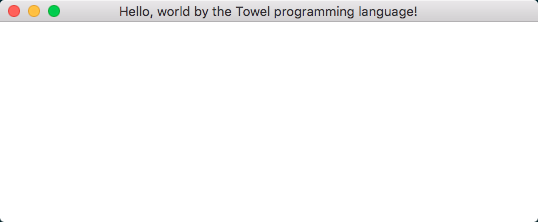
\includegraphics[scale=0.75]{fig-gui.png}
  \caption{Hello world!}
  \label{fig:gui}
\end{figure}

\part{The Towel Assembly and Virtual Machine Manual}

\chapter{An Overview on the Towel Virtual Machine}
\label{chap:tvm-overview}

The Towel virtual machine is basically a stack-based state machine that accepts and executes Towel Assembly Language. It reads instructions sequently from instruction buffer and does its computation on stacks. It has the following important parts:
\begin{itemize}
\item execution stack (or the activation record stack): \texttt{ctx\_t list}\footnote{Note that, Towel Virtual Machine does not restricts itself to any single kind of implementation. The use of OCaml type notation here is for convenience and clarity.}
\item data stack stack: \texttt{value\_t dstack\_t dstack\_t}
\item flags record: \texttt{flags\_t}
\item module table: \texttt{(module\_id\_t, module\_t) Hashtbl.t}
\item extension table: \texttt{(module\_id\_t, module TowelExtTemplate) Hashtbl.t}
\end{itemize}

\section{Execution Stack}

Execution stack is where context of function calls are stored. A context of a function call consists the return address of the function call, the module id of the return address is in\footnote{The PC jumps around different instruction arrays of different modules.}, the function value of the function being called, whether the call is made in a tail recursive fashion, etc.

When a new function call is made, the context of this call is pushed onto the execution stack, followed by the instruction pointer jumping to the start position of the function, and the \texttt{curmod} field being switched to the target module. When the instruction \texttt{ret} is met, the function returns. TVM pops the TOS on execution stack and jumps to the return address stored in this TOS and switch back to the original module according to the \texttt{ctx\_t} value.

\begin{mdframed}[style=detail]
  Execution stack has one element in it initially. This context has no
  meaningful record fields.
\end{mdframed}

\section{Data Stack Stack}

Every function has a stack for itself to do its computation. This avoids stack corruptions along all the function executions. Data stack is essentially an important part of the context of the function call, but it is so important, we would like to operate them manually so that we could be more flexible.

Normally, when a new function call is made, a new data stack is pushed onto the data stack stack. When the function returns, TVM pops the TOS from the TOS of data stack stack (i.e. the return value of this function is the TOS of current function's data stack), pushes it onto the caller's stack (next to the TOS of data stack stack). Then this data stack gets popped, thus the caller's data stack is now the TOS of the data stack stack.

\begin{mdframed}[style=detail]
  Data stack stack has one element (i.e. a data stack) in it
  initially, whereas the data stack has no elements whatsoever.

  Data stack stack is implemented by module \texttt{Nstack}, which
  provides the type \texttt{'a dstack\_t} (d for dynamic), and a lot
  of dedicated function for accessing the \texttt{dss} field in
  various ways.
\end{mdframed}

\section{Flags}

Flags stores the essential states for the virtual machine to run. For example, \texttt{curmod} records the current module whose instructions the PC is pointing at. \texttt{dss} is the data stack stack we talked about above. \texttt{scps} stores all the the names in scope stack (\texttt{scope\_t list}) for scoping.

\section{Module table}

Any functional Towel source code inevitably references (or, imports) other modules. When an \inst{import} is executing, a \texttt{module\_t} value is created and based on the module name, a UID is allocated for this module for referencing it later. Then the VM uses the UID as the key to store the \texttt{module\_t} value into the module table.

\subsection{Modules}

A module is a compiled Towel source code loaded into TVM, it has the following important fields:
\begin{itemize}
\item \texttt{id} of type \texttt{module\_id\_t}
\item \texttt{insts} of type \texttt{line array}
\item \texttt{exs} of type \texttt{(name\_t, value\_t) Hashtbl.t}
\item \texttt{imports} of type \texttt{(module\_id\_t, module\_id\_t) Hashtbl.t}
\end{itemize}

\texttt{exs} is the exported value table of the module, mapping from a name to a value.

\texttt{imports} is the absolute module id relative to this module. In the Towel compiler, names are resolved by a 2-tuple: the name id in the module and the module id. Because when compiling, the Towel compiler has no information about other modules other than the \texttt{.e} exportation file (like the header files you use in C). So it can only label other modules by IDs relative to itself (itself being zero).

When importing a new module, the module gets a global (absolute) id, all the referencing of this module should be made through this very id. So it's vital that every module maintains a mapping from the relative module id in its instructions to the absolute module id given by TVM. See \ref{fig:fig-imports} for an intuitive illustration.

\begin{figure}[h]
\psscalebox{1 1} % Change this value to rescale the drawing.
{
\begin{pspicture}(0,-6.8)(12.02,6.8)
\psframe[linecolor=black, linewidth=0.04, dimen=outer](5.62,6.8)(0.42,-2.0)
\rput[bl](1.22,4.4){\texttt{push-name 0u 1u}}
\rput[bl](1.22,4.0){\texttt{push-name 0u 2u}}
\rput[bl](1.22,3.6){\texttt{push-name 0u 0u}}
\rput[bl](1.22,5.2){\texttt{import 'std' 1u}}
\rput[bl](1.22,4.8){\texttt{import 'random' 2u}}
\rput[bl](1.22,5.6){\texttt{...}}
\rput[bl](1.22,3.2){\texttt{...}}
\psframe[linecolor=blue, linewidth=0.04, dimen=outer](12.02,6.8)(7.62,1.2)
\rput[bl](2.02,-2.4){Your module}
\rput[bl](8.82,0.8){Module Std}
\rput[bl](8.02,5.6){\texttt{...}}
\rput[bl](8.02,5.2){\texttt{bind 0u}}
\rput[bl](8.02,4.8){\texttt{...}}
\rput[bl](8.82,0.4){\texttt{id = 5u}}
\rput[bl](0.82,6.4){\texttt{id = 1u}}
\psframe[linecolor=green, linewidth=0.04, dimen=outer](12.02,-0.4)(7.62,-6.0)
\rput[bl](8.02,-3.6){\texttt{...}}
\rput[bl](8.02,-4.0){\texttt{bind 0u}}
\rput[bl](8.02,-4.4){\texttt{...}}
\rput[bl](8.82,-6.4){Module Random}
\rput[bl](8.82,-6.8){\texttt{id = 3u}}
\psframe[linecolor=black, linewidth=0.04, dimen=outer](5.22,6.0)(0.82,2.8)
\psframe[linecolor=black, linewidth=0.04, dimen=outer](5.22,1.2)(0.82,-1.2)
\rput[bl](1.22,0.8){\texttt{1u -> 5u}}
\rput[bl](1.22,0.4){\texttt{2u -> 3u}}
\rput[bl](2.42,2.4){\texttt{insts}}
\rput[bl](2.42,-1.6){\texttt{imports}}
\psline[linecolor=blue, linewidth=0.04](4.02,4.4)(4.42,4.4)(4.42,1.6)(1.22,1.6)(0.82,1.6)(0.82,0.8)(1.22,0.8)(1.22,0.8)
\psline[linecolor=blue, linewidth=0.04](2.82,0.8)(7.22,0.8)(7.22,5.2)(7.62,5.2)(7.62,5.2)
\psline[linecolor=green, linewidth=0.04](4.02,4.0)(4.82,4.0)(4.82,2.0)(0.02,2.0)(0.02,0.4)(1.22,0.4)(1.22,0.4)
\psline[linecolor=green, linewidth=0.04](2.82,0.4)(7.22,0.4)(7.22,-4.0)(7.62,-4.0)(7.62,-4.0)
\end{pspicture}
}
\caption{Illustration on the Usage of the \texttt{imports} table}
\label{fig:fig-imports}
\end{figure}

\section{Extension table}

Essentially the same thing as the module table, except that it stores extensions (of type \texttt{module Ext.TowelExtTemplate}) via \inst{load-ext}.

\renewcommand{\marg}[1]{\texttt{IARG\_#1}}
\newcommand{\sarg}[1]{\texttt{SARG\_#1}}
\newcommand{\parg}[1]{\texttt{PARG\_#1}}

\chapter{Towel Assembly Language and Its Instructions}

\section{Overview}

Towel Assembly Language has the same (or less) lexical elements as the Towel programming language. And it's grammar is very simple: each line of a Towel Assembly program has no or multiple labels, an instruction, and some arguments or no argument at all according to the instruction's arity.

After assembling, labels preceding a line are eliminated, and labels as arguments are replaced with their absolute position (i.e. the line number relative to the starting of the TAL source file, of the line where they appear as line labels).

Essentially, this assembly language is considered to be the intermediate representation of compiled Towel programs. And the TVM is a facility to execute IR directly. We can always compile IR further to, for example, native code or other virtual machines like JVM.

\subsection{Data Types}

\begin{itemize}
\item \texttt{VString}: a string surrounded by single quote
\item \texttt{VAtom}: an unsigned 64bit integer followed by an ``a''
\item \texttt{VUFixedInt}: an unsigned 64bit integer followed by a ``u''
\item \texttt{VFixedInt}: a signed 64bit integer
\item \texttt{VInt}: an integer of arbitrary precision followed by an ``l''
\item \texttt{VFloat}: a float number
\end{itemize}

\section{Scope-related Instructions}

\begin{mdframed}[style=hint]
  In the upcoming sections, we use the following convention to denote arguments of the instructions:

  \begin{itemize}
  \item \marg{SOME} means this argument is a part of an instruction.
  \item \sarg{SOME} means this argument is fetched from the data stack, and it will be put back potentially modified.

Stack argument that appears first is popped first, and so forth.

Also the term TOS and \sarg{SOME} are often interchangeable if there exists only one stack argument.
  \item \parg{SOME} is the same as \sarg{SOME}, except that \parg{SOME} is popped out from the stack forever.
  \end{itemize}
\end{mdframed}

\begin{mdframed}[style=hint]
Almost every nullary instruction is wrapper by an inline anonymous function (i.e. shared sequence) in the module \texttt{.w} so that they can be invoked. Because this is a very low-level module, so we prepend a dot to it, meaning to hide it from regular users.

Also because of its low-levelness, we can only code this module in the Towel Assembly Language, so a Ruby script \texttt{std\_gen.rb} is used to automatically generate this primitive wrapper module.

Run \texttt{ruby std\_gen.rb} and see \texttt{.w.l} and \texttt{.w.e} for detail.
\end{mdframed}

\subsection{\texttt{0x01} \inst{push-scope}}

Pushes a new scope onto the scope stack.

\subsection{\texttt{0x02} \inst{pop-scope}}

Pops the TOS of the scope stack.

\subsection{\texttt{0x03} \inst{share-scope}}

Does absolutely nothing. Just a place-holder to indicate that this new context shares the same scope with its parent.

\subsection{\texttt{0x04} \inst{bind} \marg{UID}}

The argument \marg{UID} denotes the ID of the name that the TVM will bind TOS to. Then TVM does it in current scope.

\subsection{\texttt{0x05} \inst{fun-arg} \marg{UID}}

\inst{fun-arg} is a compound instruction\footnote{A compound instruction is an instruction with multiple side-effects.}. It steals (pops) from the caller's data stack\footnote{The second top stack of DSS, or the top stack of DSS if it's a tail recursive call.} and binds a reference to the value to the name indicated by the \marg{UID} in the clone of the \texttt{closure} table of the function.

\begin{mdframed}[style=detail]
  If the stack turns out to be empty, this instruction saves the
  name-value pairs already bound (arguments stole by previous
  \inst{fun-arg}s) in the copy of the closure of the current function
  (\texttt{curfun} of the TOS of ctxs), marks the function as partial
  and returns that function.

  Also if the stack is empty because the TOS is a phony, it removes the
  phony.
\end{mdframed}

\begin{mdframed}[style=hint]
  Why copy the \texttt{closure} table? Think about the execution of a recursive function,

\begin{verbatim}
  {ctx_current with arg1 = 5; arg2 = ?}
  {ctx1 with arg1 = 3; arg2 = 4}
  {ctx0 with arg1 = 1; arg2 = 2}
\end{verbatim}

If arguments were put into the table directly, applying arg2 with, for example, 10, in \texttt{ctx\_current} will result in \texttt{ctx1.arg2 <- 10} and \texttt{ctx0.arg2 <- 10}. In other words, you just corrupted the activation records.

So you may ask, why not putting the arguments directly on stack, and bind the given \marg{UID} to the index of that argument, just like what \inst{bind} does? The reason is that, if this is the case, it would be almost impossible to implement automatic partialization. Because when returning the partial applied function, the stack that saves the arguments will be destroyed, and all your arguments will be lost.
\end{mdframed}

Sorry for such a complicated (and probably the only complicated) instruction.

\section{Stack-related Instructions}

\subsection{\texttt{0x10} \inst{push-fun} \marg{START}}

Makes a new function value and pushes it onto the stack without evaluating it. It takes \marg{START} as the start position of the function to be created. The module id of the function is considered to be \texttt{curmod.id}.

\subsection{\texttt{0x11} \inst{push-lnil} and \texttt{0x12} \inst{push-tnil}}

Makes a new list or tuple on top of the current data stack. TVM also puts the pointer of its content onto \texttt{ctx\_t.list\_make\_stack} of the top most \texttt{ctx\_t} value to keep track where to put new values (such as values from \inst{push-lit}, \inst{push-lnil} or \inst{push-tnil}), when TVM reaches \inst{end-list} or \inst{end-tuple}, the ref on top of \texttt{ctx\_t.list\_make\_stack} of the top most \texttt{ctx\_t} is popped.

\begin{mdframed}[style=detail]
  Only selected instructions have effect on these list pointers:
  \begin{itemize}
  \item \inst{eval-and-push}
  \item \inst{push-lit}
  \item \inst{push-phony}
  \item \inst{push-name}
  \item \inst{push-fun}
  \item \inst{dup}
  \item Instructions that return some value.
  \end{itemize}
\end{mdframed}

\subsection{\texttt{0x13} \inst{end-list} and \texttt{0x14} \inst{end-tuple}}

Ends current list or tuple construction.

\subsection{\texttt{0x15} \inst{push-lit} \marg{LIT}}

Pushes a literal \marg{LIT} onto the stack or the list pointer on top of \texttt{ctx\_t.list\_make\_stack}.

\subsection{\texttt{0x16} \inst{push-name} \marg{NID} \marg{MID}}

Finds the value bound to the name whose ID is \marg{NID}, in the module with the module ID being \marg{MID}, then pushes it onto the stack.

\subsection{\texttt{0x17} \inst{eval-and-push} \marg{NID} \marg{MID}}

Takes two arguments as the description of a name (same as \inst{push-name}), finds the value it is bound to. If the value is a function, then evaluates the function.

\subsection{\texttt{0x18} \inst{pop} \parg{POPPED}}

Pops the TOS of current data stack. In other words, it gets an argument from the stack, then does absolutely nothing.

\subsection{\texttt{0x19} \inst{dup} \sarg{SOME}}

Duplicates the TOS of current data stack. In other words, it gets an argument from the stack, then puts back two.

\subsection{\texttt{0x1a} \inst{reverse} \parg{N} \sarg{1} \sarg{2} ... \sarg{N} (deprecated)}

Takes an argument from the stack, then reverses the \parg{N}-top most elements.

\subsection{\texttt{0x1b} \inst{unpack} \parg{E}}

Assumes the TOS is a list or tuple, then unpacks it onto the stack.

\begin{mdframed}[style=example]
\begin{verbatim}
  dsck: [ ... | [1 2 3]]
  after unpack: [ ... | 1 | 2 | 3]
\end{verbatim}
\end{mdframed}
\subsection{\texttt{0x1c} \inst{pack} \parg{N} \parg{1} \parg{2} ... \parg{K} ...}

Takes one integer \parg{N} from the stack to pack \parg{N} items on the stack into a list. If \parg{N} is negative one, it packs all the elements on the stack until it encounters a phony, in which case the phony will be popped.

\begin{mdframed}[style=example]
\begin{verbatim}
  dsck: [ ... | 1 | 2 | 3 | 3]
  after pack: [ ... | [1 2 3]]
\end{verbatim}
\end{mdframed}

\begin{mdframed}[style=hint]
  If there were insufficient number of stack items, TVM throws an
  exception and terminates.
\end{mdframed}

\subsection{\texttt{0x1d} \inst{push-phony}}

Pushes a phony onto the stack that fakes an empty stack. That is to say, whenever TVM encounters a phony, it regards the stack as being empty.

\section{Function-related Instructions}

\subsection{\texttt{0x20} \inst{push-stack}}

Pushes a new data stack onto the data stack stack.

\subsection{\texttt{0x21} \inst{share-stack}}

Same as \inst{share-scope}.

\subsection{\texttt{0x22} \inst{pop-stack}}

Pops the current data stack.

\subsection{\texttt{0x23} \inst{eval-tail} \marg{NID} \marg{MID}}

Finds the function the two arguments references to, then calls it in a tail recursive manner.

\begin{mdframed}[style=detail]
  Some complications with the current implementation of tail recursion:
  \begin{itemize}
  \item If you use something that pushes a new scope in a tail recursion, and before this scope is popped, you tail recursed the same function again, then your scoping are leaking.

The right way to do this is to count how many scopes are pushed during this tail call context, and before the next tail call, pop as many scopes as the counter indicates.
  \item Don't remember to clear the \texttt{ctx\_t} field \texttt{list\_make\_stack}. This is likely to be ignored. However, this implies that calling a function in a tail recursive manner during a list creation will most like get you wrong results.
  \end{itemize}
\end{mdframed}

\subsection{\texttt{0x24} \inst{ret} \sarg{RET\_VAL}}

Take care of the return value of the function. Pops the execution stack. And jumps to the return address.

\begin{mdframed}[style=detail]
  The actual implementation is a bit harder than this, because you have to handle the situation where a function returns its return value into a pending list or tuple, e.g. \texttt{[(1 2 +)]}.

Also note that because we're returning control to the caller, the pending list or tuple we seek is in the caller's \texttt{ctx\_t}, i.e. second top most value of \texttt{ctxs}, rather than the TOS of \texttt{ctxs}.
\end{mdframed}


\subsection{\texttt{0x25} \inst{shared-ret}}

Just sets the instruction pointer back to where this shared sequence gets called. No return value copied whatsoever (because there isn't any).

\subsection{\texttt{0x26} \inst{closure} \marg{NID} \marg{MID} \sarg{FUN}}

Assumes \sarg{FUN} is a function, takes two argument to describe the name \sarg{FUN} should capture.

\begin{mdframed}[style=detail]
  Because you only need to capture names from self-module, so \marg{MID} is often left being zero\footnote{The self-module ID, i.e. the ID modules reference themselves to.} when compiling.
\end{mdframed}

\subsection{\texttt{0x27} \inst{invoke} \parg{FUN}}

Assumes TOS is a function, then invokes it. \parg{FUN} is popped before evaluating it.

\subsection{\texttt{0x28} \inst{call} \marg{START}}

Records $PC + 1$ as the return address, then jumps to \marg{START}.

\subsection{\texttt{0x29} \inst{install} \sarg{FUN}}

Install the captured names of \sarg{FUN} into current scope so that users can reference them.

\subsection{\texttt{0x2a} \inst{sweep}}

Sweeps the stack to get rid of all the existing elements. Used under tail recursive calls to avoid stack leakage.

\begin{mdframed}[style=hint]
  This instruction is generated for every function after all the \inst{fun-arg} instructions are finished. But it's only operational when \texttt{ctx.is\_tail\_recursive\_call} is \texttt{true}.
\end{mdframed}

\begin{mdframed}[style=hint]
  This instruction only jumps within the same module.
\end{mdframed}

\section{Conditional Branching Instructions}

\subsection{\texttt{0x30} \inst{jump} \marg{POS}}

Unconditionally jumps to \marg{POS}.

\subsection{\inst{j*} \marg{POS} \sarg{X}}

Tests the TOS with specific predicates. If the result is true, TVM jumps to \marg{POS}, otherwise, TVM executes the next instruction.

\inst{j*} instruction family consists of the following instructions:
\begin{itemize}
\item \texttt{0x32} \inst{jgz}: \sarg{X} is greater than zero,

\texttt{0x31} \inst{jgez}: \sarg{X} is greater than or equal to zero

\item \texttt{0x34} \inst{jlz}: \sarg{X} is less than zero,

\texttt{0x33} \inst{jlez}: \sarg{X} is less than or equal to zero

\item \texttt{0x35} \inst{jez}: \sarg{X} is equal to zero,

\texttt{0x36} \inst{jnez}: \sarg{X} is not equal to zero

\item \texttt{0x37} \inst{jt}: \sarg{X} is \texttt{true},

\texttt{0x38} \inst{jf}: \sarg{X} is \texttt{false}
\end{itemize}

\subsection{\inst{hj*} \marg{POS} \parg{X}}

Hungry versions of \inst{j*} instruction family, which consume the TOS they test against. Their \texttt{opcode}s are the ones of their non-hungry counterpart plus \texttt{0x10}. For example, the \texttt{opcode} of \texttt{hjgz} is \texttt{0x42}.

\subsection{\texttt{0x39} \inst{je} \marg{POS}, \texttt{0x3a} \inst{jne} \marg{POS}}

Both of them test if the data stack is empty. \inst{je} jumps to \marg{POS} if it is empty, whereas \inst{jne} jumps only when the stack is non-empty.

\begin{mdframed}[style=detail]
  If \inst{je} is tested against a phony, it pops it before branching.
\end{mdframed}

\section{Arithmetic Instructions}

\subsection{\texttt{0x50} \inst{add}, \texttt{0x51} \inst{sub}, \texttt{0x52} \inst{mul}, \texttt{0x53} \inst{div}}

Takes two arguments \parg{1} and \parg{2} from stack. Does arithmetic operations with \parg{1} and \parg{2}, and pushes \texttt{\parg{2} op \parg{1}}. These instructions work for all the number types\footnote{Atoms are not numbers.}.

\subsection{\texttt{0x55} \inst{mod} \parg{1} \parg{2}}

Does modulo operation between integer types.

\subsection{\texttt{0x56} \inst{equ} \parg{1} \parg{2}}

Does equality test on \parg{1} \parg{2}, and puts back \texttt{true} or \texttt{false} atoms.

\begin{mdframed}[style=hint]
  If two different types are tested against each other, TVM exits.
\end{mdframed}

\subsection{Bitwise Instructions}

Fixed integers, unsigned fixed integers, and big integers are supported by the following bitwise arithmetic operations:
\begin{itemize}
\item Bitwise and, \texttt{0x57} \inst{and} \parg{1} \parg{2}
\item Bitwise or, \texttt{0x58} \inst{or} \parg{1} \parg{2}
\item Bitwise xor, \texttt{0x59} \inst{xor} \parg{1} \parg{2}
\item Bitwise not, \texttt{0x5a} \inst{not} \parg{1}
\item Bitwise shift left, \texttt{0x5b} \inst{shl} \parg{X} \parg{N}
\item Bitwise shift right, \texttt{0x5c} \inst{shr} \parg{X} \parg{N}
\item Bitwise logical shift right, \texttt{0x5d} \inst{lshr} \parg{X} \parg{N}
\end{itemize}

Note that \inst{not}, \inst{and} and \inst{or} also work on the \texttt{true} and \texttt{false} atoms.

\subsection{Conversion Instructions}

These instructions allow one type of TOS to convert into value of other types. They are of the following form:
\begin{itemize}
\item \texttt{0x62} \inst{to-fint} \parg{X}
\item \texttt{0x63} \inst{to-ufint} \parg{X}
\item \texttt{0x64} \inst{to-int} \parg{X}
\item \texttt{0x65} \inst{to-float} \parg{X}
\item \texttt{0x66} \inst{to-str} \parg{X}
\end{itemize}

\section{Instructions for Enumerables}

\subsection{\texttt{0x5e} \inst{car} \parg{XS}}

Does CAR operation on linked lists and strings. It takes a list or string from the stack, puts back the head of the list or string.

\subsection{\texttt{0x5f} \inst{cdr} \parg{XS}}

Same as \inst{car}, except that it puts back the rest of the list or string.

\subsection{\texttt{0x60} \inst{cons} \parg{XS} \parg{X}}

Does CONS operation on linked lists and strings. It constructs a new list or string depending on the type of operands and then puts it back onto the stack.

\begin{mdframed}[style=hint]
  If it encounters a tuple, TVM complains and exits.
\end{mdframed}

\subsection{\texttt{0x61} \inst{list-empty} \parg{XS}}

Tests if the TOS is an empty \textbf{list, tuple or string}. It puts back whether \texttt{true} or \texttt{false}, depending on the emptiness of the list, tuple or string.

\subsection{\texttt{0xf3} \inst{tuple-at} \parg{N} \parg{XS}}

Pushes back the \parg{N}-th element of \parg{XS}.

\section{I/O Instructions}

\subsection{\texttt{0x67} \inst{show} \parg{X}}

Prints the TOS to standard output.

\subsection{\texttt{0x68} \inst{read}}

Reads a string from standard input and store that string on the stack.

\section{Extension Instructions}

\subsection{\texttt{0xf1} \inst{load-ext} \parg{EXT\_STR}}

Loads the extension by the filename of \parg{EXT\_STR} from filesystem, and records it in the \texttt{opened\_exts} table. Then puts back the handle to that extension module.

\subsection{\texttt{0xf0} \inst{extcall} \parg{EXT\_ID} \parg{EXT\_CN}}

Takes two unsigned integers from the stack. Argument \parg{EXT\_ID} is for specifying the extension module handle, the other one is the call number to indicate which routine to call from the extension.

\section{Miscellaneous Instructions}

\subsection{\texttt{0x70} \inst{import} \parg{MOD\_STR} \marg{REL\_ID}}

Finds the module by the filename of \parg{MOD\_STR} and assign it's ID relative to current ID as \marg{REL\_ID}\footnote{See previous section on modules for more details.}.

TVM will assign a unique ID to every module imported based on this \parg{MOD\_STR}. For example, the module string of module \texttt{Std} from the Towel standard library (or Towelib) is \texttt{'std'} (because the source filename of it is \texttt{'std.t'}).

\subsection{\texttt{0x7f} \inst{export} \marg{UID}}

Exports the value bound by the name ID \marg{UID} to the module's \texttt{exs} field.

\subsection{\texttt{0x71} \inst{dint}}

TVM pauses execution, and invokes the debug interrupt handler, which waits for the user to input a debug command of one line and then go on executing. Currently supported commands are
\begin{itemize}
\item \texttt{ss}: print scope stack
\item \texttt{ds}: print data stack stack
\item \texttt{vi}: print the value at given stack index.
\item \texttt{ln}: lookup the index the given name is bound to
\end{itemize}

See also \url{https://github.com/qwert42/ketivm/blob/master/vm/keti.py#L164}, which is an implementation of a similar instruction.

\subsection{\texttt{0x72} \inst{type} \parg{X}}

Pushes the type information of TOS onto the stack. This instruction only recognizes built-in types.

\subsection{\texttt{0xff} \inst{not-implemented}}

Prints an error message stating that an unimplemented instruction was found and the virtual machine has to exit.

\subsection{\texttt{0x0} \inst{idle}}

Does absolutely nothing.

\subsection{\texttt{0xfe} \inst{terminate}}

Terminate the Towel Virtual Machine. Or when finishing importing modules, go back to original module.

\begin{mdframed}[style=hint]
  Look at the similarities between (\inst{call}, \inst{invoke},
  etc. \texttt{->} \inst{ret}) and (\inst{import} \texttt{->}
  \inst{terminate}).
\end{mdframed}

\chapter{Bytecode Form of the Towel Assembly Language}

\section{Bytecode Form Overview}

A Towel Assembly Language source code can be compiled into a binary file. The layout of such a binary file is as follows:
\begin{itemize}
\item Magic number \texttt{0x4242}, denotes that this is a Towel binary
\item The data segment, which contains all the literals used in the original source code
\item Magic number \texttt{0xff3080ff}, denotes that data segment ends here
\item The code segment
\end{itemize}

\section{Data Segment}
A Towel binary contains only one data segment. Data segment contains all the literals used in the original source code file, which are of type \texttt{VString}, \texttt{VAtom}, \texttt{VFixedInt}, \texttt{VUFixedInt}, \texttt{VInt}, \texttt{VFloat}.

To store a string in the data segment. First, put a tag\footnote{Actually a string.} \texttt{``s''} into the data segment. After that tag, put a little endian 32-bit unsigned integer which represents the length of the string. Then put the contents of the string after the 32-bit integer.

To store an atom, put a tag \texttt{``a''} and then an unsigned little endian 64-bit integer.

To store a fixed integer, put a tag \texttt{``f''}, then a signed little endian 64-bit integer.

An unsigned fixed integer is the same as an atom, except the tag is \texttt{``u''}.

To store an integer (i.e. big integer) or a float, put their respective tags (\texttt{``b''} for integer, \texttt{``n''}\footnote{``n'' for not a number.} for float) before their binary string representations.

\begin{mdframed}[style=example]
  For a float \texttt{3.14159}, the Towel literal binary
  representation is \texttt{6e07000000332e3134313539}.
\end{mdframed}


The order of the literals are put in the data segment is their respective labels.

\section{Instruction Format}

Any bytecode instruction is a little-endian 64 bit number. The first byte of the number is \texttt{opcode}. For unary instructions, the second up to eighth bytes consists of the argument label. For binary instructions, the second up to fifth bytes consists of the first argument label, while the rest (sixth to eigth, 3 bytes, less than the first argument) consists of the second argument label.

When encountered a bytecode instruction, use the argument labels (if any) to retrieve actual arguments from data segment, and then form the actual instruction.

\begin{mdframed}[style=example]
  Suppose we have the following bytecode file:

\begin{verbatim}
  BB
    s03000000std
    u0100000000000000
    u0200000000000000
    s12000000Hello, world
    u1500000000000000
  ff3080ff

  1501000000000000
  7002000000000000
  1703000000050000
  1504000000000000
  fe00000000000000
\end{verbatim}

First, we can identify this file as a Towel bytecode because the first two bytes are \texttt{0x4242}, i.e. \texttt{BB}.

We also know that there are 5 literals in the data segment:
\begin{enumerate}
\item a string: \texttt{'std'}
\item an unsigned fixed integer 1
\item an unsigned fixed integer 2
\item a string: \texttt{'Hello, world'}
\item an unsigned fixed integer 0x15
\end{enumerate}

Then, for the first instruction (8 bytes), we get \texttt{opcode} from the first byte, in this case, \texttt{0x15}, which is \inst{push-lit} with \marg{LIT}, so we reinterpret from the 2nd to the 8th byte as an integer, 1. And get an element from the data segment by the index of one, which turns out to be the \texttt{'std'} string.\footnote{Yes, the index of data segment starts from one.}

So we can finally reconstruct the first instruction to be \texttt{PUSH\_LIT('str')}.

Now let's look at the third instruction, we lookup the \texttt{opcode} \texttt{0x17} is \inst{eval-and-push} with \marg{NID} and \marg{MID}, so we reinterpret from the 2nd to the 5th byte as an integer, i.e. 3, and 6th to 8th as another integer, 5.

Thus the two arguments are \texttt{2} and \texttt{0x15}. So we can also reconstruct this instruction to be\newline \texttt{EVAL\_AND\_PUSH(2, 0x15)}. The rest instructions are the same.

\end{mdframed}

\begin{mdframed}[style=detail]
  One of the neat things about this kind of representation is that I don't have to modify the assembler even when I have variable-sized instructions, because the addresses I'm jumping to are counted by instructions from the start, rather than bytes.
\end{mdframed}

\chapter{Extending the Towel Virtual Machine (OCaml Implementation)}

By using the Extension interface (in \texttt{src/vm/ext.ml}), you can easily add new functionalities to TVM, enabling more powerful Towel programming experience.

\section{Prerequisite}

The library (no matter if it's third-party, or of your own) should be \textbf{OCaml-compliant}, because TVM is built on top of OCaml too. That is to say, you should be able to write OCaml programs with it, thus TVM will have access to it via dynamic linking.

\begin{mdframed}[style=hint]
  I think plain C libraries with only thin OCaml wrappers (no
  \texttt{ml} files) would work too. Because \texttt{Dynlink} only
  needs it to be a OCaml-aware shared-library.
\end{mdframed}

\section{Approach}

Two instructions were implemented in TVM: \inst{load-ext} and \inst{extcall}.

\inst{load-ext} takes an \texttt{ext\_str} from the stack and loads the corresponding extension module into TVM via the OCaml standard module \texttt{Dynlink}. An \texttt{ext\_str} is a filename of the OCaml object file. After successfully loading it, the instruction leaves an unsigned integer (\texttt{OVUFixedInt}) on the stack for future reference of the extension.

\begin{mdframed}[style=hint]
   \texttt{ext\_str} should always ends with \texttt{.cmo} even if the target is a \texttt{.cmxs} file.
\end{mdframed}

\inst{extcall} takes two arguments from the stack: it first takes the TOS as the extension handle (the one \inst{load-ext} pushed), then it takes another unsigned integer as the extension function call number (although this integer will be converted into an OCaml \texttt{int}, but I think $2^{31}$ is fairly enough for ordinary libraries). The extension module then matches against the call number to determine which action to perform on the data stack.

\section{Howto}

\begin{mdframed}[style=hint]
  The following step illustrates how to build native extension rather
  than bytecode extension. If you want bytecode extension, use
  \texttt{ocamlc} instead, and probably lose some of the parameters.
\end{mdframed}

The first step, create a OCaml plugin. This plugin file is essentially a dynamic library (e.g. a \texttt{.so} file on *nix, a \texttt{.dll} file on Windows). When implementing this plugin, you must implement the module interface \texttt{TowelExtTemplate} laid out in \texttt{src/vm/ext.ml}. It's simple: one function - \texttt{extcall}. You will have to route individual call numbers to different routines using this function.

The first argument of \texttt{extcall} is the call number, then the second one is the \texttt{dss} of the VM, for you to get specific arguments from the data stack or leave your results on it. But be careful, if you ruin this dss, the TVM is doomed.

After you finish your \texttt{extcall} function and other local functions, remember to register your module value in the \texttt{\_\_ext\_\_} slot so that when loading this extension, TVM will get to know of your extension.

The second step, you compile your source code via the following command:

\begin{mdframed}[style=example]
  \texttt{ocamlfind ocamlopt -package \%1 \%2 -shared -linkall -I \%3
    -o \%4}
\end{mdframed}
Of these parameters:
\begin{itemize}
\item (\texttt{\%1}) the packages your extension module uses, take \texttt{ext\_random.ml} as an example, \texttt{\%1} will be replaced by stdint;
\item (\texttt{\%2}) the extension module source file, \texttt{ext\_random.ml}, for example;
\item (\texttt{\%3}) the directory where \texttt{t.cmi} and \texttt{nstack.cmi} are;
\item (\texttt{\%4}) the output binary filename, \texttt{ext\_random.cmxs}, for exmpale;
\item If you use some libraries that are not included in standard library, you may want to use \texttt{-linkpkg} instead of \texttt{-linkall} (for example, when building binding library for Tk).
\end{itemize}

The command for compiling the Random extension module is like this:

\begin{mdframed}[style=example]
  \texttt{ocamlfind ocamlopt -package stdint ext\_random.ml -shared
    -linkall -I ../../build/src/vm -o ext\_random.cmxs}
\end{mdframed}

Third, place the \texttt{.cmxs} file in the \texttt{libpaths} of TVM, default locations are current working directory and the folder \texttt{towelib}. Modify \texttt{src/vm/config.ml} to change these locations.

Last, write a Towel wrapper module for your extension module. In the \texttt{.w} instruction wrapper module, name \texttt{!>ext} is bound to the \inst{load-ext} instruction wrapper and name \texttt{!>>} for \inst{extcall}. You should always bind a name to the extension handle pushed by \texttt{!>ext}.

\begin{mdframed}[style=hint]
  It is often a good idea to bind a local partial applied function with the handle already applied to \texttt{!>>}.
\end{mdframed}

\part[The Implementation of the Project]{The Implementation of the Project\footnote{Special thanks to Professor Edwards for so many valuable suggestions.}}

\chapter{Project Plan}

\section{A Little Bit of History about Towel}
The original idea of Towel was to create an esoteric programming language like \textit{Shakespear} or \textit{Piet}. The central idea was that every program structure is identified by the first character. For example, \texttt{if} \texttt{is} \texttt{is-not} are all recognized as an \texttt{IF} token. With this tokenizer, you could write a GCD program in a lorem-ipsum manner.

But this soon turned out to be infeasible when you want to name more than 26 things. So the one-character grammar idea got abandoned.

But still, I want to create something different, especially in the way the programs will look like. So I thought to myself, we already have the Lisp family (prefix), as well as the ML family (infix). Let's do postfix!\footnote{At that time, I didn't realize that there are so many postfix languages already!} Soon the idea of stack-based postfix-syntaxed functional language came into being. Then I named it after my favorite novel series.

\section{Specification and Development Process}

Specification was not clear at the beginning of the development, but became clearer and clearer as the development went on.

The three of us get together every Monday afternoon before meeting with Professor Edwards. We would discuss the newly implemented parts and ideas, and hoped this discussion would clearify things for them as well as myself, and identify as much flaws as possible. Then during the week, new parts would get developed, and flaws fixed.

Later in the development (after the test suite was implemented as well as several test cases), the development process began to be like Test-Driven Development spontaneously.

Manuals (or specification) were modified along development (at least for the first month) to fit what we had at that time. Later in the development, because features got added or redone too fast, they quickly went out of date, and finally got a major revision after feature freeze.

\section{Testing Process}

After each major feature was completed, one or two test cases would be created to test if the feature would work.

Not long before feature freeze, some holistic test cases were made to ensure everything works correctly together. Such test cases include, for example, \texttt{quicksort.t} for quicksort and \texttt{adv-obj.t} for advanced OO simulation. It was during these tests, some serious defects were discovered, for example, scope leakage due to unbalanced \inst{pop-scope} instruction during code generation for sequences\footnote{Fixed in commit \texttt{adb1d3c752}.}, or improperly designed data structure in the virtual machine that causes function calls in list literals to return the return value to wrong location\footnote{Fixed in commit \texttt{ccdf962de7}.}.

After the feature freeze, tests are still being added to the test suite.

\section{Programming Style}

Basically, we used Unix-style naming conventions, i.e. underscores.

The whole indentation rule we used was the default configuration of \texttt{ocp-indent}.

Particularly,

\begin{itemize}
\item No lines should exceed 80 characters wide.
\item Append \texttt{\_t} to most type names.
\item \texttt{in} clause starts at the second line of that
  \texttt{let-in} expression.
\item \texttt{then} and \texttt{else} clause both starts a new line, i.e.
  \begin{minted}{ocaml}
    if something
    then some_other_thing
    else something_else
  \end{minted}
\item Prefer \texttt{begin} and \texttt{end} over parentheses.
\item Modularize the source files: the functions contained in one OCaml file should only serve one purpose. Except some modules, such as \texttt{Common}.
\item \texttt{let}, \texttt{try}, \texttt{if}, and \texttt{match} starts right after \texttt{in}, \texttt{then}, or \texttt{else}:
  \begin{minted}{ocaml}
    let x = Some(1)
    in if something
      then try if something
               then ahh
               else ohh
           with Error ->
             raise Failure
      else match a with
          Some(x) -> x
        | None -> raise NothingHere
  \end{minted}
\end{itemize}

\section{Project Timeline}

We had no designated project timeline whatsoever. By the time I consider the language to have become stable\footnote{Although I fixed another several severe bugs later.}, it was about just right about two weeks before the report due. We got lucky.

Here's the major changes made in the code repository:

\begin{itemize}
\item Sep 24: THE Initial Commit.
\item Sep 27: Proposal commited.
\item Oct 9: Somewhat working scanner and parser.
\item Oct 20: LRM commited.
\item Nov 8: Got a working compiler.
\item Nov 15: Hello world!
\item Nov 17: Towel standard library commited.
\item Nov 29: Major change to the VM.
\item Dec 3: Extension mechanism added to the VM.
\item Dec 4: The language become dynamic officially (dynatowel branch merged into master).
\item Dec 6: Bytetowel merged.
\item Dec 11: Feature freeze.
\end{itemize}

\section{Roles and Responsibilities}

\begin{itemize}
\item Project Manager: None
\item The Guru Guy: Zihang Chen
\item System Architect: Zihang Chen
\item Testers: Zihang Chen, Baochan Zheng, Guanlin Chen
\end{itemize}

\section{Tools and Languages Used in Developemnt}

\begin{itemize}
\item OCaml 4.02.

\item \texttt{opam} for installing OCaml packages, \texttt{findlib} for compiling my source code with the packages, and \texttt{ocamldebug} for some information on stack trace. Overall package usage: \texttt{Batteries}, \texttt{Stdint}, \texttt{Sha}, \texttt{Extlib}, \texttt{menhir}.

\item Emacs 24.5 with \texttt{tuareg-mode} (OCaml syntax
  highlighting), \texttt{merlin} (syntax and semantics checking,
  linting) and \texttt{ocp-indent} (indenting OCaml). These are
  recommended by the \texttt{opam} official website.

\item Ruby 2.2.3 is used for test automation and compiler/VM source code
  generation (to write as less boilerplate code as possible).

\item Waf (a Python3 tool) is used as the building framework of the
  project, Python3 is used for the building script.

\item \XeTeX{} for document compilation and AUCTeX for \LaTeX ~editing.

\item Git for project version control, GitHub for project hosting, and Google for some of the problem solving. English for understanding the OCaml and Batteries manual, also the solutions I found on Stackoverflow.
\end{itemize}

\section{Project Log}

See Appendix \autoref{project-log}.

\chapter{Architectural Design}

\section{Overall}

In this chapter, we consider the term intermediate representation to be synonymous with the term Towel Assembly.

\begin{figure}[H]
  \centering
  \begin{tikzpicture}[ roundnode/.style={circle, draw=green!60,
      fill=green!5, very thick, minimum size=3cm},
    squarednode/.style={rectangle, draw=red!60, fill=red!5, very
      thick, minimum size=3cm}, ]
    % Nodes
    \node[squarednode] (sourcecode) {Source code}; \node[roundnode]
    (compiler) [right=of sourcecode] {Compiler}; \node[squarednode]
    (ir) [below right=-0.5cm and 1cm of compiler] {IR}; \node[roundnode] (vm) [below=of
    compiler] {Virtual Machine}; \node[squarednode] (output) [left=of
    vm] {42};
    % Lines
    \draw[->] (sourcecode.east) -- (compiler.west); \draw[->]
    (compiler.east) -- (ir.north); \draw[->] (ir.south) -- (vm.east);
    \draw[->] (vm.west) -- (output.east);
  \end{tikzpicture}

  \caption{Overall Architecture}
  \label{fig:overall}
\end{figure}

\section{Structural Overview on the Towel Compiler (Zihang Chen)}

  The compiler frontend (module \texttt{Weave}) first invokes \texttt{Switches.parse} to parse the switch configuration for the source code. Then it gets the abstract syntax tree out of the source code by tokenizing and parsing it with modules \texttt{Scanner.token} and \texttt{Parser.sentence}.

  After that, it invokes module \texttt{Compile.compile} to transform the AST data structure to the AST of intermediate representation. While traversing the AST, module \texttt{Compile} also makes use of module \texttt{Scoping} to do scope analysis and report any names that get referenced to without first binding something to it. If such name is found, the compilation aborts immediately.

  \begin{mdframed}[style=detail]
    Module \texttt{Cseg} defines an infix operator \texttt{(|\mtilde ~\mtilde ~|)} to represent the concatenation of two \texttt{Tasm\_ast.asm} data structures into one. This greatly simplifies the work for code generation. Because you can write the code generation part in a really straight-forward way, like this:
    \begin{minted}[linenos]{ocaml}
      let snippet = cnil
                    |~~| preamble
                    |~~| (line INSTALL)
                    |~~| fun_args
                    |~~| (line SWEEP)
                    |~~| body_inst
                    |~~| (cline [end_label] (Some(POP_SCOPE)))
                    |~~| (line RET)
                    |~~| (put_label [real_end_label])

    \end{minted}

    The \texttt{Compile.compile} function basically takes a \texttt{Sentence}, then for each word in the \texttt{Sentence}, it invokes \texttt{g\_word}. For each kind of word, \texttt{g\_word} route them to respective \texttt{g\_*} functions. For each kind of word, there exists a corresponding \texttt{g\_*} function.

Each \texttt{g\_*} function takes a parameter \texttt{ctx} to keep track of the current context of the code generation, for example, the scope environment the piece of AST is in, or if the piece of AST is backquoted, etc.

Some of the \texttt{g\_*} functions (specifically, those words that represents a single value, for example, literals, sequences, etc) also take another parameter \texttt{inst\_ctx} for the \texttt{g\_bind} function to generate proper \inst{bind} instruction.

  \end{mdframed}

  With the IR AST, the compiler invokes \texttt{Assemble.assemble} to get rid of all the labels, and replace them with absolute positions. After this step, the compiler gets Assembled IR AST.

  In the last step, the compiler invokes \texttt{Tasm\_bytecode.b\_asm} to procure the bytecode representation of the IR.

  \begin{mdframed}[style=hint]
  The above mainly talked about the very common invocation to the compiler, for other uses, for example, outputing text version of Assembled IR AST, the compiler uses \texttt{Tasm\_stringify.p\_asm}.

  See also \autoref{fig:compiler-arch}.
  \end{mdframed}

\begin{figure}[htbp]
  \centering
  \begin{tikzpicture}[ roundnode/.style={circle, draw=green!60,
      fill=green!5, very thick, minimum size=2cm},
    squarednode/.style={rectangle, draw=red!60, fill=red!5, very
      thick, minimum size=2cm}, ]
    % Nodes
    \node[squarednode] (sourcecode) {Source code}; \node[roundnode]
    (switches) [right=of sourcecode] {Switches.parse};
    \node[roundnode] (scanner) [right=of switches] {Tokenize};
    \node[roundnode] (parser) [right=of scanner] {Parse};
    \node[squarednode] (parsed_ast) [below left=1.2cm and 0cm of
    parser] {AST}; \node[roundnode] (compile) [below=of parsed_ast]
    {Compile}; \node[squarednode] (ast_ir) [below=of compile] {IR
      AST}; \node[roundnode] (assemble) [below left=1.2cm and 0cm of
    ast_ir] {Assemble}; \node[roundnode] (stringify_raw) [below
    right=1.2cm and 0cm of ast_ir] {Stringify}; \node[squarednode]
    (raw) [below right=of stringify_raw] {Raw IR}; \node[roundnode]
    (ir_stringify) [below left=1.2cm and 0cm of assemble] {Stringify};
    \node[squarednode] (asm_ir) [below=of ir_stringify] {Assembled
      IR}; \node[roundnode] (bytecode) [below right=1.2cm and 0cm of
    assemble] {Bytecode}; \node[squarednode] (bc_ir) [below=of
    bytecode] {Bytecode IR};
    % Lines
    \draw[->] (sourcecode.east) -- (switches.west); \draw[->]
    (switches.east) -- (scanner.west); \draw[->] (scanner.east) --
    (parser.west); \draw[->] (parser.south west) --
    (parsed_ast.north); \draw[->] (parsed_ast.south) --
    (compile.north); \draw[->] (compile.south) -- (ast_ir.north);
    \draw[->] (ast_ir.south) -- (assemble.north east); \draw[->]
    (ast_ir.south) -- (stringify_raw.north west); \draw[->]
    (assemble.south) -- (ir_stringify.north east); \draw[->]
    (assemble.south) -- (bytecode.north west); \draw[->]
    (stringify_raw.south east) -- (raw.north west); \draw[->]
    (ir_stringify.south) -- (asm_ir.north); \draw[->] (bytecode.south)
    -- (bc_ir.north);
  \end{tikzpicture}
  \caption{Compiler Architecture}
  \label{fig:compiler-arch}
\end{figure}

\section{Structural Overview on the Towel Virtual Machine (Zihang Chen)}

Things are much simpler on the VM-side. The virtual machine frontend \texttt{Tvm} first reads in the bytecode representation of IR, transforms it back into IR AST by invoking \texttt{Tasm\_inv\_bytecode.parse\_bytecode}. Then invokes \texttt{Nvm.exec} to execute all the instructions parsed. \texttt{Nvm.exec} is a simple wrapper function to bootstrap \texttt{Nvm.\_\_exec}, which actually does all the work.

The function \texttt{Nvm.\_\_exec} implements all the instructions available in a very big \texttt{match} expression. After each execution of an instruction, it tail calls itself with the new state of the virtual machine (for example, \texttt{flags}, IP, etc.) to execute the next instruction pointed by IP. For more on the state of the Towel Virtual Machine, see also \autoref{chap:tvm-overview}.

For certain instructions that are quite alike, for example, the arithmetic instructions and branching instructions, we use Ruby scripts to generate respective code for them, then invoke them in \texttt{Nvm.exec}.\footnote{An alternative to do this is by \texttt{camlp4}.}

\begin{mdframed}[style=detail]
The \texttt{Nvm.exec} depends on many other functions from other modules to work. For example,

\begin{itemize}
\item The module \texttt{T} provides all the basic data types for the TVM, an example would be the value type \texttt{T.value\_t}.

\item The module \texttt{Vm\_t} provides various data types specific for this implementation of the TVM, such as \texttt{Vm\_t.flags\_t}.

\item The module \texttt{Nstack} provides support for the stack data
  structure and various operations used by \texttt{Nvm.exec}.

\item The module \texttt{Arithmetics} provides implementation for various arithmetics instructions.

\item The module \texttt{Jumps} provides \texttt{Jumps.branch} to do branching.

\item The module \texttt{Dscoping} provides data structure and operations for scoping.

\item The module \texttt{Ext} implements extension (plugin) mechanism for \inst{load-ext} and \inst{extcall}.
\end{itemize}
\end{mdframed}

\begin{figure}[htbp]
  \centering
  \begin{tikzpicture}[ roundnode/.style={circle, draw=green!60,
      fill=green!5, very thick, minimum size=2cm},
    squarednode/.style={rectangle, draw=red!60, fill=red!5, very
      thick, minimum size=2cm}]
    \node[squarednode] (bc_ir) {Bytecode IR};
    \node[roundnode] (bc_inv) [below=of bc_ir] {Bytecode Parser};
    \node[squarednode] (ir_ast) [below=of bc_inv] {IR AST};
    \node[roundnode] (exec) [below=of ir_ast] {\texttt{exec}};
    \node[squarednode] (output) [below=of exec] {Output};
    \node[squarednode] (mods) [below right=0cm and 1cm of ir_ast] {Other Bytecode Modules};
    \node[roundnode] (ext_) [below left=0cm and 1cm of ir_ast] {\texttt{ext.ml}};
    \node[squarednode] (exts) [below right=0cm and 1.3cm of exec] {Other Extension Modules};
    \node[roundnode] (nstack) [below left=0cm and 1.3cm of exec] {...};
    \draw[->] (bc_ir.south) -- (bc_inv.north);
    \draw[->] (bc_inv.south) -- (ir_ast.north);
    \draw[->] (ir_ast.south) -- (exec.north);
    \draw[->] (exec.south) -- (output.north);
    \draw[->] (mods.west) -- (exec.east);
    \draw[->] (ext_.east) -- (exec.west);
    \draw[->] (nstack.east) -- (exec.west);
    \draw[->] (exts.west) -- (exec.east);
  \end{tikzpicture}
  \caption{Virtual Machine Architecture}
  \label{fig:vm-arch}
\end{figure}

\section{The Towel Assembly Components (Zihang Chen)}

The script \texttt{ccg.rb} generates a whole bunch of Towel Assembly related modules for the compiler or the virtual machine to generate bytecode or parse text form IR.

The generated modules include:
\begin{itemize}
\item \texttt{tasm\_ast.mli}

defines abstract syntax tree types

\item \texttt{tasm\_scanner.mll}

scanner for text form IR

\item \texttt{tasm\_parser.mly}

parser for text form IR

\item \texttt{tasm\_stringify.ml}

provides functions for converting AST to human-readable string

\item \texttt{tasm\_bytecode.ml}

provides functions for converting AST to VM-readable bytecode

\item \texttt{tasm\_inv\_bytecode.ml}

provides functions for parsing bytecode back to AST
\end{itemize}

\begin{mdframed}[style=detail]
  The \texttt{ccg.rb} script reads information on the instructions from the accompanied Ruby script \texttt{inst.rb}. So when tweaking instructions for the Towel Assembly Language, only \texttt{inst.rb} is changed.
\end{mdframed}

\chapter{Test Plan}

\section{Individual Test Examples}

\subsection{\texttt{partial.t}}
\begin{mdframed}[style=cl]
\begin{verbatim}
  "---
  Tests partial function application.
  !>>
  !<< 42
  41
  [2 2]
  "

  import 'std' \

  bind Dec1 (1 -\Std)
  then (43 Dec1 !println\Std 42 Dec1 !println\Std)
\end{verbatim}
\end{mdframed}

The raw text form of the IR is as follows:

\begin{mdframed}[style=cl]
\begin{verbatim}
  push-stack
  push-scope
  push-lit 'std'
  import 1u
  push-scope
  call :6e59cf543-1u-st
  bind 1u
  push-lit 43
  eval-and-push 1u 0u
  eval-and-push 25u 1u
  push-lit 42
  eval-and-push 1u 0u
  eval-and-push 25u 1u
  pop-scope
  terminate
:6e59cf543-1u-st push-stack
  push-lit 1
  eval-and-push 4u 1u
:6e59cf543-1u-end ret
:6e59cf543-1u-real-end
\end{verbatim}

Raw text form IR are trivial. We won't show more of these.
\end{mdframed}

The assembled text form of the IR is as follows:

\begin{mdframed}[style=cl]
\begin{verbatim}
  push-stack
  push-scope
  push-lit 'std'
  import 1u
  push-scope
  call 15u
  bind 1u
  push-lit 43
  eval-and-push 1u 0u
  eval-and-push 25u 1u
  push-lit 42
  eval-and-push 1u 0u
  eval-and-push 25u 1u
  pop-scope
  terminate
  push-stack
  push-lit 1
  eval-and-push 4u 1u
  ret
\end{verbatim}
\end{mdframed}

The assembled binary form of the IR is as follows:

\begin{mdframed}[style=cl]
\begin{verbatim}
  4242 7303 0000 0073 7464 7501 0000 0000
  0000 0075 0f00 0000 0000 0000 662b 0000
  0000 0000 0075 0000 0000 0000 0000 7519
  0000 0000 0000 0066 2a00 0000 0000 0000
  6601 0000 0000 0000 0075 0400 0000 0000
  0000 ff30 80ff 2000 0000 0000 0000 0100
  0000 0000 0000 1501 0000 0000 0000 7002
  0000 0000 0000 0100 0000 0000 0000 2803
  0000 0000 0000 0402 0000 0000 0000 1504
  0000 0000 0000 1702 0000 0005 0000 1706
  0000 0002 0000 1507 0000 0000 0000 1702
  0000 0005 0000 1706 0000 0002 0000 0200
  0000 0000 0000 fe00 0000 0000 0000 2000
  0000 0000 0000 1508 0000 0000 0000 1709
  0000 0002 0000 2400 0000 0000 0000
\end{verbatim}
\end{mdframed}

\subsection{\texttt{bind.t}}

\begin{mdframed}[style=cl]
\begin{verbatim}
  "---
  Tests if nested bind and also works.
  !>>
  !<< 3
  -1
  5
  3
  10
  -2
  9
  3
  12
  11
  "

  import 'std' \

  bind A fun` B,
    bind C fun` D,
      bind E (1 2 -\Std)
      then (((E !println\Std D !println\Std B !println\Std 10)))
    also F fun` D,
      bind E (5 7 -\Std)
      then (E !println\Std D !println\Std B !println\Std 12)
    then (B !println\Std 5 C !println\Std 9 F !println\Std 11)
  then (3 A !println\Std)
\end{verbatim}
\end{mdframed}

The assembled text form of the IR is as follows:

\begin{mdframed}[style=cl]
\begin{verbatim}
   push-stack
   push-scope
   push-lit 'std'
   import 1u
   push-scope
   push-fun 12u
   bind 1u
   push-lit 3
   eval-and-push 1u 0u
   eval-and-push 25u 1u
   pop-scope
   terminate
   push-stack
   push-scope
   install
   fun-arg 2u
   push-scope
   push-fun 57u
   bind 3u
   closure 2u
   push-fun 35u
   bind 6u
   closure 2u
   eval-and-push 2u 0u
   eval-and-push 25u 1u
   push-lit 5
   eval-and-push 3u 0u
   eval-and-push 25u 1u
   push-lit 9
   eval-and-push 6u 0u
   eval-and-push 25u 1u
   push-lit 11
   pop-scope
   pop-scope
   ret
   push-stack
   push-scope
   install
   fun-arg 4u
   push-scope
   call 52u
   bind 5u
   eval-and-push 5u 0u
   eval-and-push 25u 1u
   eval-and-push 4u 0u
   eval-and-push 25u 1u
   eval-and-push 2u 0u
   eval-and-push 25u 1u
   push-lit 12
   pop-scope
   pop-scope
   ret
   push-stack
   push-lit 5
   push-lit 7
   eval-and-push 4u 1u
   ret
   push-stack
   push-scope
   install
   fun-arg 4u
   push-scope
   call 80u
   bind 5u
   call 68u
   pop-scope
   pop-scope
   ret
   push-stack
   call 71u
   ret
   push-stack
   eval-and-push 5u 0u
   eval-and-push 25u 1u
   eval-and-push 4u 0u
   eval-and-push 25u 1u
   eval-and-push 2u 0u
   eval-and-push 25u 1u
   push-lit 10
   ret
   push-stack
   push-lit 1
   push-lit 2
   eval-and-push 4u 1u
   ret
\end{verbatim}
\end{mdframed}

The assembled binary form of the IR is as follows:

\begin{mdframed}[style=cl]
\begin{verbatim}
  4242 7303 0000 0073 7464 7501 0000 0000
  0000 0075 0c00 0000 0000 0000 6603 0000
  0000 0000 0075 0000 0000 0000 0000 7519
  0000 0000 0000 0075 0200 0000 0000 0000
  7539 0000 0000 0000 0075 0300 0000 0000
  0000 7523 0000 0000 0000 0075 0600 0000
  0000 0000 6605 0000 0000 0000 0066 0900
  0000 0000 0000 660b 0000 0000 0000 0075
  0400 0000 0000 0000 7534 0000 0000 0000
  0075 0500 0000 0000 0000 660c 0000 0000
  0000 0066 0700 0000 0000 0000 7550 0000
  0000 0000 0075 4400 0000 0000 0000 7547
  0000 0000 0000 0066 0a00 0000 0000 0000
  6601 0000 0000 0000 0066 0200 0000 0000
  0000 ff30 80ff 2000 0000 0000 0000 0100
  0000 0000 0000 1501 0000 0000 0000 7002
  0000 0000 0000 0100 0000 0000 0000 1003
  0000 0000 0000 0402 0000 0000 0000 1504
  0000 0000 0000 1702 0000 0005 0000 1706
  0000 0002 0000 0200 0000 0000 0000 fe00
  0000 0000 0000 2000 0000 0000 0000 0100
  0000 0000 0000 f200 0000 0000 0000 0507
  0000 0000 0000 0100 0000 0000 0000 1008
  0000 0000 0000 0409 0000 0000 0000 2607
  0000 0000 0000 100a 0000 0000 0000 040b
  0000 0000 0000 2607 0000 0000 0000 1707
  0000 0005 0000 1706 0000 0002 0000 150c
  0000 0000 0000 1709 0000 0005 0000 1706
  0000 0002 0000 150d 0000 0000 0000 170b
  0000 0005 0000 1706 0000 0002 0000 150e
  0000 0000 0000 0200 0000 0000 0000 0200
  0000 0000 0000 2400 0000 0000 0000 2000
  0000 0000 0000 0100 0000 0000 0000 f200
  0000 0000 0000 050f 0000 0000 0000 0100
  0000 0000 0000 2810 0000 0000 0000 0411
  0000 0000 0000 1711 0000 0005 0000 1706
  0000 0002 0000 170f 0000 0005 0000 1706
  0000 0002 0000 1707 0000 0005 0000 1706
  0000 0002 0000 1512 0000 0000 0000 0200
  0000 0000 0000 0200 0000 0000 0000 2400
  0000 0000 0000 2000 0000 0000 0000 150c
  0000 0000 0000 1513 0000 0000 0000 170f
  0000 0002 0000 2400 0000 0000 0000 2000
  0000 0000 0000 0100 0000 0000 0000 f200
  0000 0000 0000 050f 0000 0000 0000 0100
  0000 0000 0000 2814 0000 0000 0000 0411
  0000 0000 0000 2815 0000 0000 0000 0200
  0000 0000 0000 0200 0000 0000 0000 2400
  0000 0000 0000 2000 0000 0000 0000 2816
  0000 0000 0000 2400 0000 0000 0000 2000
  0000 0000 0000 1711 0000 0005 0000 1706
  0000 0002 0000 170f 0000 0005 0000 1706
  0000 0002 0000 1707 0000 0005 0000 1706
  0000 0002 0000 1517 0000 0000 0000 2400
  0000 0000 0000 2000 0000 0000 0000 1518
  0000 0000 0000 1519 0000 0000 0000 170f
  0000 0002 0000 2400 0000 0000 0000
\end{verbatim}
\end{mdframed}

\section{Holistic Test Example: Quicksort}

\begin{mdframed}[style=cl]
\begin{verbatim}
  "---
  Holistic test: Quicksort.
  !>>
  !<< [1 2 3 4 5]
  "

  import 'std' \

  bind #quicksort ,\ L,
    (L ?#empty\Std ift (!!pop\Std []), (!!pop\Std
      bind ~h (L #hd\Std)
      also ~t (L #tl\Std)
      then (~t (~h >\Std) /filter\Std #quicksort
            [~h]
            ~t (~h <=\Std) /filter\Std #quicksort
        #concat\Std #concat\Std)))
  then ([5 4 3 2 1] #quicksort !println\Std)
\end{verbatim}
\end{mdframed}

The assembled text form of the IR is as follows:

\begin{mdframed}[style=cl]
\begin{verbatim}
  push-stack
  push-scope
  push-lit 'std'
  import 1u
  push-scope
  push-fun 19u
  bind 1u
  closure 1u
  push-lnil
  push-lit 5
  push-lit 4
  push-lit 3
  push-lit 2
  push-lit 1
  end-list
  eval-and-push 1u 0u
  eval-and-push 25u 1u
  pop-scope
  terminate
  push-stack
  push-scope
  install
  fun-arg 2u
  eval-and-push 2u 0u
  eval-and-push 36u 1u
  jf 30u
  eval-and-push 27u 1u
  push-lnil
  end-list
  jump 50u
  eval-and-push 27u 1u
  push-scope
  call 64u
  bind 3u
  call 60u
  bind 4u
  eval-and-push 4u 0u
  call 56u
  eval-and-push 59u 1u
  eval-and-push 1u 0u
  push-lnil
  eval-and-push 3u 0u
  end-list
  eval-and-push 4u 0u
  call 52u
  eval-and-push 59u 1u
  eval-and-push 1u 0u
  eval-and-push 57u 1u
  eval-and-push 57u 1u
  pop-scope
  pop-scope
  ret
  push-stack
  eval-and-push 3u 0u
  eval-and-push 13u 1u
  ret
  push-stack
  eval-and-push 3u 0u
  eval-and-push 10u 1u
  ret
  push-stack
  eval-and-push 2u 0u
  eval-and-push 32u 1u
  ret
  push-stack
  eval-and-push 2u 0u
  eval-and-push 30u 1u
  ret
\end{verbatim}
\end{mdframed}

The assembled binary form of the IR is as follows:

\begin{mdframed}[style=cl]
\begin{verbatim}
  4242 7303 0000 0073 7464 7501 0000 0000
  0000 0075 1300 0000 0000 0000 6605 0000
  0000 0000 0066 0400 0000 0000 0000 6603
  0000 0000 0000 0066 0200 0000 0000 0000
  6601 0000 0000 0000 0075 0000 0000 0000
  0000 7519 0000 0000 0000 0075 0200 0000
  0000 0000 7524 0000 0000 0000 0075 1e00
  0000 0000 0000 751b 0000 0000 0000 0075
  3200 0000 0000 0000 7540 0000 0000 0000
  0075 0300 0000 0000 0000 753c 0000 0000
  0000 0075 0400 0000 0000 0000 7538 0000
  0000 0000 0075 3b00 0000 0000 0000 7534
  0000 0000 0000 0075 3900 0000 0000 0000
  750d 0000 0000 0000 0075 0a00 0000 0000
  0000 7520 0000 0000 0000 00ff 3080 ff20
  0000 0000 0000 0001 0000 0000 0000 0015
  0100 0000 0000 0070 0200 0000 0000 0001
  0000 0000 0000 0010 0300 0000 0000 0004
  0200 0000 0000 0026 0200 0000 0000 0011
  0000 0000 0000 0015 0400 0000 0000 0015
  0500 0000 0000 0015 0600 0000 0000 0015
  0700 0000 0000 0015 0800 0000 0000 0013
  0000 0000 0000 0017 0200 0000 0900 0017
  0a00 0000 0200 0002 0000 0000 0000 00fe
  0000 0000 0000 0020 0000 0000 0000 0001
  0000 0000 0000 00f2 0000 0000 0000 0005
  0b00 0000 0000 0017 0b00 0000 0900 0017
  0c00 0000 0200 0038 0d00 0000 0000 0017
  0e00 0000 0200 0011 0000 0000 0000 0013
  0000 0000 0000 0030 0f00 0000 0000 0017
  0e00 0000 0200 0001 0000 0000 0000 0028
  1000 0000 0000 0004 1100 0000 0000 0028
  1200 0000 0000 0004 1300 0000 0000 0017
  1300 0000 0900 0028 1400 0000 0000 0017
  1500 0000 0200 0017 0200 0000 0900 0011
  0000 0000 0000 0017 1100 0000 0900 0013
  0000 0000 0000 0017 1300 0000 0900 0028
  1600 0000 0000 0017 1500 0000 0200 0017
  0200 0000 0900 0017 1700 0000 0200 0017
  1700 0000 0200 0002 0000 0000 0000 0002
  0000 0000 0000 0024 0000 0000 0000 0020
  0000 0000 0000 0017 1100 0000 0900 0017
  1800 0000 0200 0024 0000 0000 0000 0020
  0000 0000 0000 0017 1100 0000 0900 0017
  1900 0000 0200 0024 0000 0000 0000 0020
  0000 0000 0000 0017 0b00 0000 0900 0017
  1a00 0000 0200 0024 0000 0000 0000 0020
  0000 0000 0000 0017 0b00 0000 0900 0017
  0d00 0000 0200 0024 0000 0000 0000 00
\end{verbatim}
\end{mdframed}

\section{The Test Suite Script: Prefect (Zihang Chen)}

When Prefect is invoked, it automatically searches the current working directory for files with extension \texttt{.t}. For each \texttt{.t} file, if the filename starts with two underscores, it is simply ignored.

The test input and expected output are all embedded in the comments of their respective test case files:

\begin{mdframed}[style=detail]
\begin{verbatim}
  "Some optional background or rationale description of this test case.
  ---
  Mandatory test case description.
  !>> optional test input
  !<< optional expected output"
\end{verbatim}

Again, we are using the exclamation mark to denote the side-effected outer world.
\end{mdframed}

A test is said to be passed if and only if it exits normally and prints to the standard output exactly the expected output.

\begin{mdframed}[style=cl]
  \begin{minted}{ruby}
#! /usr/bin/env ruby

require 'open3'
require 'colorize'

class Prefect
  # This class tests per file.
  IN_PREFIX = '!>> ?'
  OUT_PREFIX = '!<< ?'

  PAT = /.*".*---\n(.*)\n#{IN_PREFIX}([^"]*)\n#{OUT_PREFIX}([^"]*)"/m
  # This means that a testcase description consists of three parts:
  # (1) the text description part that tells what this testcase is about
  # (2) the input part, led by !>>\space
  # (3) the expected output part, led by !<<\space

  def initialize(fp, **ctx)
    @ctx = ctx
    @fp = fp.chop.chop

    open(fp) {|f|
      @content = f.read
    }

    extract_info
  end

  def extract_info
    matches = PAT.match(@content)
    unless matches.nil?
      @description, @input, @expected_output = matches.captures
      @description.strip!
    end
  end

  def execute_ok(idx)
    pretty_input = if @input == ''
                     'None'.light_cyan
                   else
                     @input.white
                   end
    pretty_output = if @expected_output == ''
                      'None'.light_cyan
                    else
                      @expected_output.white
                    end

    puts "Testcase #{('#' + idx.to_s).blue}: #{@description}
---
Input: #{pretty_input}
Output: #{pretty_output}"

    out, err, status = Open3.capture3(@ctx[:weave_path],
                                    "#{@fp}.t",
                                    '-o',
                                    "temp/#{@fp}.w")

    if status.exitstatus != 0
      [false, out]
      return
    end

    if ARGV[0] == '-t'
      puts "Tracing #{@fp}.w =>"
      output, _ = Open3.capture2(
          @ctx[:tvm_path], "temp/#{@fp}.w", '-t', :stdin_data=>@input
      )
    else
      output, err, status = Open3.capture3(
          @ctx[:tvm_path], "temp/#{@fp}.w", :stdin_data=>@input
      )
    end

    if status.exitstatus != 0
      [false, err]
      return
    end

    if output == @expected_output
      [true, output]
    else
      [false, output]
    end
  end
end

if __FILE__ == $0
  require 'fileutils'
  FileUtils.remove_entry_secure 'temp'
  FileUtils.mkdir 'temp'

  SUFFIX = 't'
  WEAVE_PATH = '../build/src/compiler/weave'
  TVM_PATH = '../build/src/vm/tvm'
  make_prefect = lambda {|fp| Prefect.new(
    fp,
    :weave_path=>WEAVE_PATH,
    :tvm_path=>TVM_PATH
  )}

  cnt = 0
  results = {}
  Dir.foreach '.' do |entry|
    if entry =~ /[^.]*\.#{SUFFIX}/
      if entry.start_with? '__'
        next
      end

      cnt += 1
      ok, out = make_prefect.call(entry).execute_ok cnt

      puts "Real output: #{out}\n"
      if ok
        results[entry] = :ok
        puts "#{entry} =====> #{'[OK]'.green}"
      else
        results[entry] = :failed
        puts "#{entry} =====> #{'[FAILED]'.red}"
      end

      puts '-' * 42
    end
  end

  count = results.inject({:ok => 0, :failed => 0}) do |acc, kv|
    _, v = kv
    acc[v] += 1
    acc
  end

  if count != {}
    if count[:ok] > 0
      ok = count[:ok].to_s.green
    else
      ok = 0.to_s
    end

    if count[:failed] > 0
      failed = count[:failed].to_s.red
    else
      failed = 0.to_s
    end
    puts "Summary: #{ok} passed, #{failed} failed."
  end
end
  \end{minted}
\end{mdframed}

\section{Tests Overview (Zihang Chen)}

16 tests were included in the test suite.

\begin{itemize}
\item \texttt{bind.t}

tests whether nested \texttt{bind} forms and \texttt{also} clauses work or not.

\item \texttt{functional.t}

tests some of the functional features of Towel, for example, partial function application.

\item \texttt{gcd.t}

tests if tail recursion and chained \texttt{if} forms work.

\item \texttt{idle.t}

tests if \texttt{.idle} works.

\item \texttt{ift-iff.t}

tests whether \texttt{ife}, \texttt{ifne}, \texttt{ift}, \texttt{iff} and phonies work.

\item \texttt{import.t}

tests whether implicit import and explicit import work as expected.

\item \texttt{list.t}

tests various functions for enumerables, for example, \mstd{\#hd}, \mstd{\#1}, etc.

\item \texttt{macro.t}

tests if shared sequences work, also tests the expressiveness of Towel.

\item \texttt{obj.t}

mimic an object-oriented programming situation, intended as testing for function closures.

\item \texttt{partial.t}

tests if partial function application is stable.

\item \texttt{phony.t}

tests if phony, partial function application and \mstd{!invoke} can work together.

\item \texttt{quicksort.t}

a holistic test, tests if non-tail recursion, the stability (whether something leaks or not) of \texttt{bind-then} forms in non-tail recursive environment, list functions, and the overall stability of the virtual machine.

\item \texttt{rnd.t}

tests if the extension mechanism of the virtual machine works.

\item \texttt{test.t}

the hello world test.

\item \texttt{zip.t}

tests if complicated list creation works (especially, function calls inside list literals) and the stability of tail recursions.

\end{itemize}

\chapter{Lessons Learned}

\section{Zihang Chen}

First of all, OCaml is great (but not perfect). Be patient and learn how to program in it. It will change your life (for someone who hasn't been doing much functional programming).

Discuss your ideas with your teammates, explain your code to people, fix your bugs right away. Keep a memo at hand, even before sleep.

If you cannot explain your idea or code to others, you don't understand them at all.

Don't be afraid to rewrite 90\% of your code. Make sure every time you do this, you reduce 10\% of the code.

You'll never get to fix all your bugs.

\subsection{Some Practical Advices}
\begin{enumerate}
\item RTFM!! It is hard to understand even the words in them at first, but you'll get to the gist after reading them for 10 times.

\item Code style matters.

\item Remember to quote your data type constructor and its arguments with a pair of parentheses when working with function application. The OCaml compiler is really stupid about this: \texttt{some\_function Some(x)}. The right way to do it is \texttt{some\_function (Some x)}, or \texttt{some\_function (Some(x))}. There are many other traps like this that will ruin a whole day for you, so watch out!

\item Use GitHub to host your code, enjoy the little deep green squares in your Contributions chart.

\item Use \texttt{opam}, \texttt{Batteries} and \texttt{Findlib}. Learn to program OCaml in Emacs, or at least Vim. Never program in Sublime Text.

\item When in trouble, first use \texttt{ocamldebug} to see the backtrace and identify the line number where your program blows up. Then use print to debug. (And maybe the time travel feature of \texttt{ocamldebug}.)\footnote{Because OCaml loses most of the type information after compilation, you can't really get something useful out of the debugger.}

\item Always wrap \texttt{Hashtbl.find} in a \texttt{try} expression, because it's really frustrating to see only a \texttt{Failure: Not\_found} printed when your program runs into trouble.

\item Don't panic.
\end{enumerate}

\section{Baochan Zheng}

Working on this unique project with a smart student is really challenging.

  The most important thing I learnt this semester is that communication is
extremely important for a teamwork task. From the very beginning, we should
have argued more about our project and make it more achievable for us. Besides,
although we stick to meeting at least once a week, we are so used to listening to
Zihang’s idea and doing things he told us to, but never challenge him. This bad
habit makes us took lots of detours, for example we’ve been to “data stack stack
stack” things and wasted a lot of time on “object reference table” which is proved
to be an inefficient way.

  On the other hand, although we spent almost the whole semester in struggling
to follow Zihang’s crazy idea, we do learn a lot from him. He showed us how to
make a language general-purpose, how to make it efficient and elegant. And we
tried to build our own virtual machine (although our coding on virtual machine
was updated by Zihang after a essential change on basic structure), which is the
thing many other groups are not working on. What’s more, we even learnt the
basic rules of Ruby to finish the module coding. We gained deep understanding
on runtime environment, stack management and other things mentioned in
class.

  Losing control of my own project doesn’t feel good, but I’m still happy about
having this chance to work with Zihang, and engaging in this crazy project.

\section{Guanlin Chen}

From the whole semester, under the tutoring of PLT class, we implemented what we learned and brought the knowledge into the real world. Towel language is a stack based programming language which roots in our team leader Zihang's mind. The logic of the programming language is complicated and requires comprehensively analysis, neatly blueprint, also intelligence.

Together with Baochan, my work focuses on the virtual machine part. Even dealing with a minor part of the whole language , I am sometimes struggled to figure out the logic and the method to construct the VM. Impressively, the 'four stack' ages was the most challenging days, CTXS, DSS, SCPS and ORT were resemble to four distinct resource station, only a properly combination could figure the desired output. Even ORT is rejected at last because of our task to simplize the language, that part of work is also a memory segment which embedded deeply in my heart. For instance, the DSS stores the reference , which is the key of the harsh table, pointing at the data. During the programming, I always mistook the real value with the reference, which gave a inproper output.

So always be logical thinking and be preoccupied when implementing something in your intricate logic. So as Zihang mentioned, 'Everytime your program confuses you, check whether the type could match.'

Another significant portion for the VM is the introduction of ruby. The basic notion occurs during the optimation of the VM. When dealing with the AST given by parser, huge amount of instructions are required, however, some of them have similar function and less distinguished programming methods. Ruby is resemble to a glue which could build script for our program to make some optimization. For the mathematics instructions portion of Towel, we should implement different mathematics operations, 'plus', 'substract', 'multiple', 'divide' for the parameters with the types like 'int', 'fint' etc...From the original method, we should deal with each of the operator with each of the type, that is time consuming and mechanical repetition tasks,once some parts should be modified, it is trivial to modify all the program. In ruby, a 'map' function could be employed to "glue" different parts by visiting all the elements from a list. This method is introduced to 'math', 'to', 'jmp'related instructions.

\part{The Future}

Although the project has accomplished most of the goals it set at the very beginning, there's still much that's left to be improved or done. For example, a native compiler that compile the intermediate representation to C code, and then procure a native application using \texttt{gcc} or \texttt{clang}.

What's more challenging, is to design a statically typed Towel. Static-typed stack-based language are rare because of their dynamic nature: a function's effect on the stack (or to put it in a StrongForth term, stack-effect) is generally not known until it is executed. So statically typing Towel will require information we don't usually define in value-based languages, namely, how many elements will be pushed (or popped, depending on the semantics of the function) after it finishes, and all their types. Type inferring is possible as well, but I suspect that the Hindly-Milner type system won't work here without any modification.

Other from the ideas above, currently, compilation error messages on the compiler-side are still very vague. It may be necessary to rewrite the compiler the fourth time to plug in line number tracing or something like that. Error handling on the VM-side is also considered very weak. Adding some kind of error recovery mechanism seems useful.

Better debugging facilities need to be implemented. Unlike OCaml, Towel is a dynamic language, there are still much information to use for debugging purposes at runtime.

There are also still large parts missing in the standard library, for example, file I/O, mutable data structure (arrays, etc.), string manipulation functions, regular expression, networking, and so on.

\begin{appendices}
\chapter[Project Log]{Project Log \footnote{Up to only feature freeze. Bug-fix commits may not have been included.}}
\label{project-log}

\input{../play/log.tex}

\chapter{Full Code Listing}

\section{License Information}

This project is licensed under the terms of BSD 3-Clause License.

\begin{verbatim}
Copyright (c) 2015, Zihang Chen (qwert42, chsc4698@gmail.com)
All rights reserved.

Redistribution and use in source and binary forms, with or without
modification, are permitted provided that the following conditions are met:

1. Redistributions of source code must retain the above copyright notice,
this list of conditions and the following disclaimer.

2. Redistributions in binary form must reproduce the above copyright notice,
this list of conditions and the following disclaimer in the documentation
and/or other materials provided with the distribution.

3. Neither the name of the copyright holder nor the names of its contributors
may be used to endorse or promote products derived from this software without
specific prior written permission.

THIS SOFTWARE IS PROVIDED BY THE COPYRIGHT HOLDERS AND CONTRIBUTORS "AS IS"
AND ANY EXPRESS OR IMPLIED WARRANTIES, INCLUDING, BUT NOT LIMITED TO, THE
IMPLIED WARRANTIES OF MERCHANTABILITY AND FITNESS FOR A PARTICULAR PURPOSE
ARE DISCLAIMED. IN NO EVENT SHALL THE COPYRIGHT HOLDER OR CONTRIBUTORS BE
LIABLE FOR ANY DIRECT, INDIRECT, INCIDENTAL, SPECIAL, EXEMPLARY, OR
CONSEQUENTIAL DAMAGES (INCLUDING, BUT NOT LIMITED TO, PROCUREMENT OF
SUBSTITUTE GOODS OR SERVICES; LOSS OF USE, DATA, OR PROFITS; OR BUSINESS
INTERRUPTION) HOWEVER CAUSED AND ON ANY THEORY OF LIABILITY, WHETHER IN
CONTRACT, STRICT LIABILITY, OR TORT (INCLUDING NEGLIGENCE OR OTHERWISE)
ARISING IN ANY WAY OUT OF THE USE OF THIS SOFTWARE, EVEN IF ADVISED OF THE
POSSIBILITY OF SUCH DAMAGE.
\end{verbatim}
\begin{mdframed}[style=hint]
  Source code is also available online at \url{https://github.com/qwert42/Towel}.
\end{mdframed}

\input{../play/xxx.tex}

\renewcommand\bibname{References}

\begin{thebibliography}{9}
\bibitem{haskell-report}

Simon Marlow. \textit{Haskell 2010 Language Report}. \url{https://www.haskell.org/onlinereport/haskell2010/}, 2015-12-16.

\bibitem{gcc-manual}
The GNU Project. \textit{The GNU C Reference Manual}.
\url{http://www.gnu.org/software/gnu-c-manual/gnu-c-manual.html}, 2015-12-12.

\bibitem{ocaml-manual}
Xavier Leroy, Damien Doligez, Alain Frisch, Jacques Garrigue, Didier Rémy and Jérôme Vouillon. \textit{The OCaml System Release 4.02 - Documentation and User's Manual}.
\url{http://caml.inria.fr/pub/docs/manual-ocaml/}, 2015-12-12.

\bibitem{forth}
J.V. Noble. \textit{A Beginner's Guide to Forth}. \url{http://galileo.phys.virginia.edu/classes/551.jvn.fall01/primer.htm}, 2015-12-12.

\bibitem{strongforth}
Stephan Becher. \textit{Introduction to StrongForth}. \url{http://www.arestlessmind.org/2009/02/03/intro.html}, 2015-12-12.

\bibitem{postscript}
Paul Bourke. \textit{PostScript Tutorial}. \url{http://paulbourke.net/dataformats/postscript/}. 2015-12-12.

\bibitem{joylang}
\textit{Joy (programming language)}. \url{https://en.wikipedia.org/wiki/Joy\_(programming\_language)}. 2015-12-12.

\bibitem{joyofjoy}
Language Perils. \textit{The Joy of Joy}. \url{http://ncreep.github.io/language\_perils/blog/2013-03-18-the-joy-of-joy.html}. 2015-12-12.

\bibitem{ocaml-libref}
Xavier Leroy, Damien Doligez, Alain Frisch, Jacques Garrigue, Didier Rémy and Jérôme Vouillon. \textit{The OCaml Library Reference}. \url{http://caml.inria.fr/pub/docs/manual-ocaml/libref/index.html}, 2015-12-12.

\bibitem{batteries-manual}
The OCaml Batteries Team. \textit{Batteries User Guide}. \url{http://ocaml-batteries-team.github.io/batteries-included/hdoc2/}, 2015-12-12.

\bibitem{funk}
Naser AlDuaij, Senyao Du, Noura Farra, Yuan Kang, Andrea Lottarini. \textit{Funk Programming Language Final Report}. \url{http://www.cs.columbia.edu/~sedwards/classes/2012/w4115-fall/reports/Funk.pdf}, 2015-12-12.
\end{thebibliography}

\end{appendices}

\end{document}
